\documentclass[12pt,a4paper]{article}
\usepackage[T1]{fontenc}
\usepackage[utf8]{inputenc}
\usepackage{lmodern}
\usepackage{mathtools,amssymb,booktabs,longtable,array,microtype}
\usepackage[dvipsnames]{xcolor}
\usepackage[a4paper,margin=24mm,headheight=16pt,headsep=9mm,footskip=12mm]{geometry}
\usepackage{tikz}
\usetikzlibrary{arrows.meta,calc}
\usepackage{caption,fancyhdr,hyperref,enumitem,needspace}
\usepackage{titlesec,tocloft,setspace,listings}
\usepackage[most]{tcolorbox}
\hypersetup{colorlinks=true,linkcolor=MidnightBlue,urlcolor=MidnightBlue,
 pdftitle={A tutorial on fixed-order convex touring polygons and directional last-step maps},
 pdfauthor={TouringPolygons project}}
\definecolor{ink}{HTML}{223247}
\definecolor{navy}{HTML}{274568}
\definecolor{pOne}{HTML}{3677AD}
\definecolor{pTwo}{HTML}{C78A24}
\definecolor{good}{HTML}{007E72}
\definecolor{bad}{HTML}{B53E62}
\definecolor{quiet}{HTML}{617384}
\definecolor{codebg}{HTML}{F3F7FA}
\definecolor{codekw}{HTML}{005D78}
\definecolor{codefun}{HTML}{315DAD}
\color{ink}
\tikzset{>=Latex,polyA/.style={draw=pOne,fill=pOne!9,line width=.9pt},
polyB/.style={draw=pTwo,fill=pTwo!10,line width=.9pt},
route/.style={draw=good,line width=1.4pt},wrong/.style={draw=bad,dashed,line width=1pt},
aux/.style={draw=quiet,dashed,line width=.8pt},smalllabel/.style={font=\scriptsize,
fill=white,fill opacity=.9,text opacity=1,inner sep=1pt}}
\setlength{\parindent}{0pt}\setlength{\parskip}{8pt}
\setlength{\emergencystretch}{2em}
\setstretch{1.09}
\setlength{\textfloatsep}{18pt plus 4pt minus 3pt}
\setlength{\intextsep}{16pt plus 4pt minus 3pt}
\captionsetup{font=small,labelfont={bf,color=navy},skip=7pt}
\titleformat{\section}{\Large\bfseries\color{navy}}{\thesection}{.75em}{}
\titleformat{\subsection}{\large\bfseries\color{good}}{\thesubsection}{.7em}{}
\titlespacing*{\section}{0pt}{23pt plus 5pt minus 3pt}{10pt}
\titlespacing*{\subsection}{0pt}{17pt plus 4pt minus 2pt}{7pt}
\renewcommand{\cfttoctitlefont}{\Large\bfseries\color{navy}}
\setlength{\cftbeforetoctitleskip}{0pt}
\setlength{\cftaftertoctitleskip}{9pt}
\setlength{\cftbeforesecskip}{3pt}
\setlength{\cftbeforesubsecskip}{0pt}
\setlength{\cftsecnumwidth}{9mm}
\setlength{\cftsubsecindent}{9mm}
\setlength{\cftsubsecnumwidth}{12mm}
\renewcommand{\cftsecfont}{\small\bfseries\color{navy}}
\renewcommand{\cftsecpagefont}{\small\bfseries\color{good}}
\renewcommand{\cftsubsecfont}{\small\color{quiet}}
\renewcommand{\cftsubsecpagefont}{\small\color{quiet}}
\renewcommand{\cftsecleader}{\cftdotfill{2}}
\renewcommand{\cftsubsecleader}{\cftdotfill{2}}
\pagestyle{fancy}\fancyhf{}
\fancyhead[L]{\small\sffamily\color{navy} DIRECTIONAL TOURING-POLYGON MAPS}
\fancyhead[R]{\small\sffamily\color{quiet} A visual implementation guide}
\fancyfoot[L]{\small\color{quiet}TouringPolygons / 14 September 2026}
\fancyfoot[R]{\small\color{navy}\thepage}
\renewcommand{\headrulewidth}{.4pt}
\newcommand{\norm}[1]{\lVert#1\rVert}
\newcommand{\R}{\mathbb R}
\newcommand{\cross}{\mathbin{\times}}
\newcommand{\code}[1]{{\ttfamily\color{codekw}#1}}
\lstdefinelanguage{TPPPseudo}{
  sensitive=true,
  morekeywords={if,else,for,while,return,skip,throw,require,not,and,or,in,has,each,append,mark,cache,copy,reverse,construct,replace,remove,sort,unique},
  morekeywords=[2]{PUBLIC_SOLVE,SPLIT_BOUNDARIES,LEX_SIGN,INSIDE_CLOSED,BUILD_VERTEX,LOCATE,VIRTUAL_SOURCE,QUERY_PATH,QUERY_LENGTH,CONE,EDGE_PLUS,CROSS_SIGN,REFLECT_POINT,REFLECT_QUERY,REFLECT_DIRECTION},
  comment=[l]{//}
}
\lstdefinestyle{tpppseudo}{
  language=TPPPseudo,
  basicstyle=\ttfamily\small,
  keywordstyle=\color{codekw}\bfseries,
  keywordstyle=[2]\color{codefun}\bfseries,
  commentstyle=\color{quiet}\itshape,
  backgroundcolor=\color{codebg},
  frame=single,rulecolor=\color{navy!25},frameround=tttt,
  framesep=4mm,xleftmargin=6mm,xrightmargin=2mm,
  numbers=left,numberstyle=\tiny\color{quiet},numbersep=7pt,
  breaklines=true,breakatwhitespace=true,columns=fullflexible,
  keepspaces=true,showstringspaces=false,aboveskip=12pt,belowskip=13pt
}
\lstnewenvironment{pseudo}{\lstset{style=tpppseudo}}{}
\newtcolorbox{sourcebox}{enhanced,breakable,colback=navy!4,colframe=navy!25,
  borderline west={2.4pt}{0pt}{good},boxrule=.4pt,arc=1mm,
  left=3mm,right=3mm,top=2.2mm,bottom=2.2mm,
  before skip=9pt,after skip=12pt,fontupper=\small}
\newtcolorbox{coverbox}{enhanced,colback=navy!4,colframe=navy!20,
  boxrule=.4pt,arc=1.5mm,left=5mm,right=5mm,top=4mm,bottom=4mm}
% All drawings are native, reproducible TikZ vectors.  Geometry panels use
% identical x/y units; panels marked schematic depict decisions, not a claimed
% complete subdivision of a particular input.
\tikzset{coordgrid/.style={draw=quiet!24,line width=.25pt}}

% Reading map: recursive actions and their queries, not a claimed cell proof.
\newcommand{\figoverview}{%
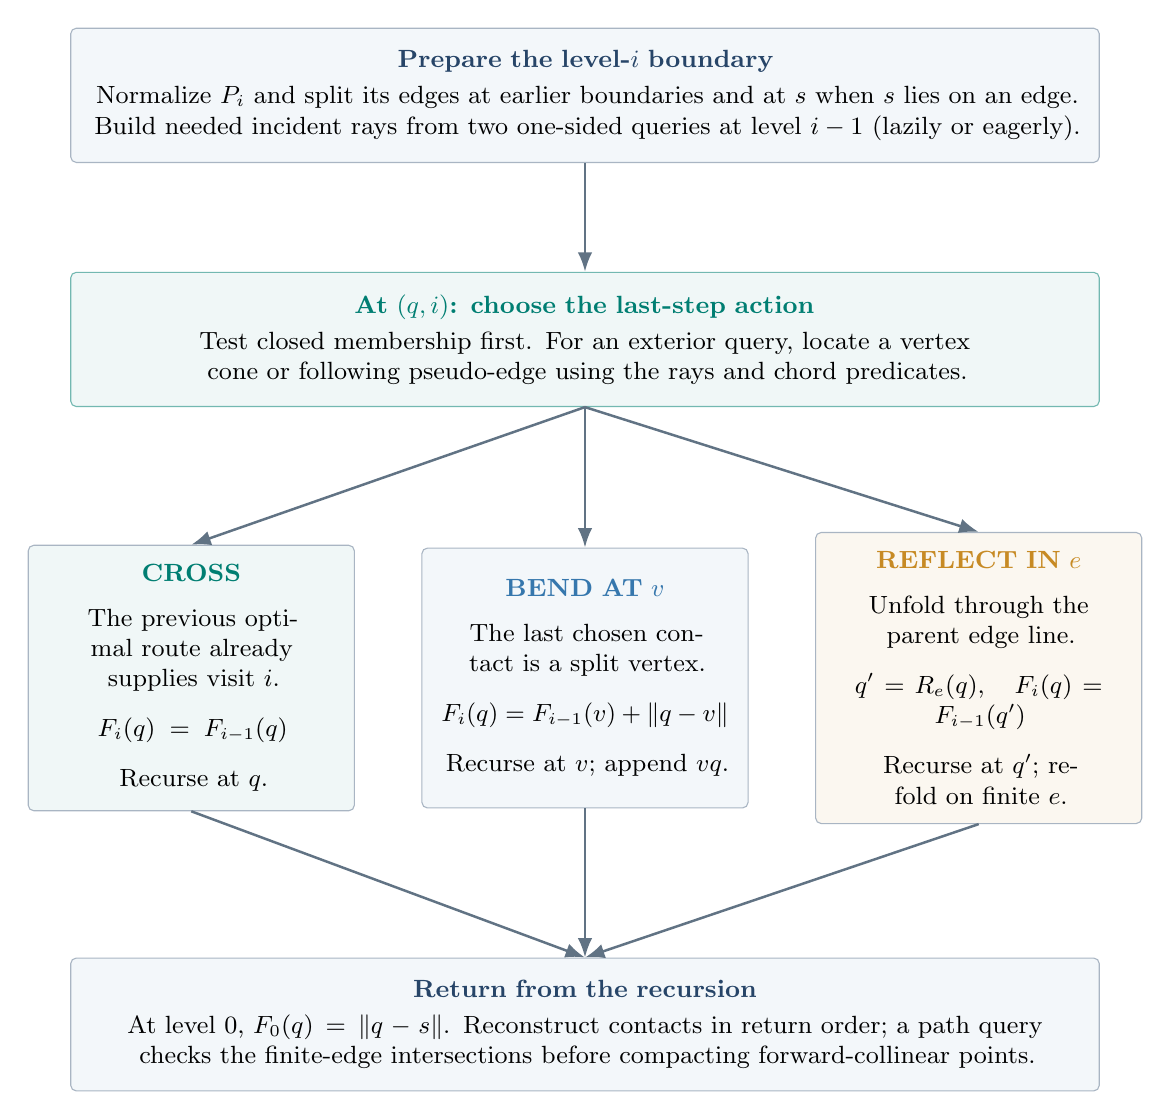
\begin{tikzpicture}[font=\small,
 overview/.style={draw=navy!40,fill=codebg,rounded corners=2pt,
   text width=12.5cm,align=center,inner sep=8pt},
 action/.style={draw=navy!40,fill=white,rounded corners=2pt,
   text width=3.65cm,minimum height=3.3cm,align=center,inner sep=7pt}]
\node[overview] (prep) at (0,0) {%
  {\bfseries\color{navy}Prepare the level-\(i\) boundary}\\[2pt]
  Normalize \(P_i\) and split its edges at earlier boundaries and at \(s\)
  when \(s\) lies on an edge.
  Build needed incident rays from two one-sided queries at level \(i-1\)
  (lazily or eagerly).};
\node[overview,fill=good!6,draw=good!55] (loc) at (0,-3.1) {%
  {\bfseries\color{good}At \((q,i)\): choose the last-step action}\\[2pt]
  Test closed membership first. For an exterior query, locate a vertex cone
  or following pseudo-edge using the rays and chord predicates.};
\node[action,fill=good!6] (crossing) at (-5,-7.4) {%
  {\bfseries\color{good}CROSS}\\[5pt]
  The previous optimal route already supplies visit \(i\).\\[7pt]
  \(F_i(q)=F_{i-1}(q)\)\\[7pt]
  Recurse at \(q\).};
\node[action,fill=pOne!6] (bend) at (0,-7.4) {%
  {\bfseries\color{pOne}BEND AT \(v\)}\\[5pt]
  The last chosen contact is a split vertex.\\[7pt]
  \(F_i(q)=F_{i-1}(v)+\|q-v\|\)\\[7pt]
  Recurse at \(v\); append \(vq\).};
\node[action,fill=pTwo!7] (reflect) at (5,-7.4) {%
  {\bfseries\color{pTwo}REFLECT IN \(e\)}\\[5pt]
  Unfold through the parent edge line.\\[7pt]
  \(q'=R_e(q),\quad F_i(q)=F_{i-1}(q')\)\\[7pt]
  Recurse at \(q'\); refold on finite \(e\).};
\node[overview] (base) at (0,-11.8) {%
  {\bfseries\color{navy}Return from the recursion}\\[2pt]
  At level \(0\), \(F_0(q)=\|q-s\|\). Reconstruct contacts in return order;
  a path query checks the finite-edge intersections before compacting
  forward-collinear points.};
\draw[quiet,-Latex,line width=.9pt] (prep.south)--(loc.north);
\foreach \target in {crossing,bend,reflect}
  \draw[quiet,-Latex,line width=.9pt] (loc.south)--(\target.north);
\foreach \target in {crossing,bend,reflect}
  \draw[quiet,-Latex,line width=.9pt] (\target.south)--(base.north);
\end{tikzpicture}}

\newcommand{\figreflection}{%
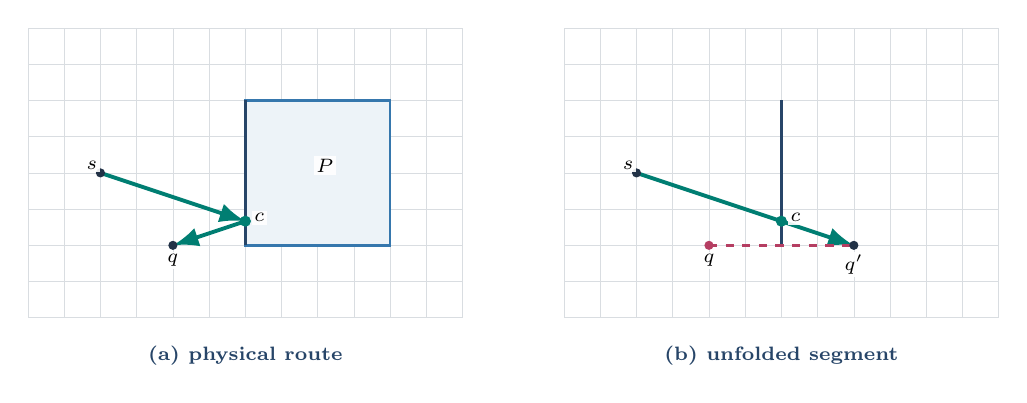
\begin{tikzpicture}[scale=.92]
\begin{scope}
  \draw[coordgrid] (-3,-1) grid[step=.5] (3,3);
  \draw[polyA] (0,0) rectangle (2,2);
  \draw[very thick,navy] (0,0)--(0,2);
  \draw[route,-Latex] (-2,1)--(0,1/3);
  \draw[route,-Latex] (0,1/3)--(-1,0);
  \fill[ink] (-2,1) circle (1.8pt);
  \fill[ink] (-1,0) circle (1.8pt);
  \fill[good] (0,1/3) circle (2.2pt);
  \node[smalllabel,above left] at (-2,1) {\(s\)};
  \node[smalllabel,below] at (-1,-.08) {\(q\)};
  \node[smalllabel,right] at (.08,.38) {\(c\)};
  \node[smalllabel] at (1.1,1.1) {\(P\)};
  \node[font=\scriptsize\bfseries,color=navy] at (0,-1.52)
    {(a) physical route};
\end{scope}
\begin{scope}[xshift=7.4cm]
  \draw[coordgrid] (-3,-1) grid[step=.5] (3,3);
  \draw[very thick,navy] (0,0)--(0,2);
  \draw[route,-Latex] (-2,1)--(1,0);
  \draw[wrong,dashed] (-1,0)--(1,0);
  \fill[ink] (-2,1) circle (1.8pt);
  \fill[bad] (-1,0) circle (1.8pt);
  \fill[good] (0,1/3) circle (2.2pt);
  \fill[ink] (1,0) circle (1.8pt);
  \node[smalllabel,above left] at (-2,1) {\(s\)};
  \node[smalllabel,below] at (-1,-.08) {\(q\)};
  \node[smalllabel,right] at (.08,.38) {\(c\)};
  \node[smalllabel,below] at (1,-.08) {\(q'\)};
  \node[font=\scriptsize\bfseries,color=navy] at (0,-1.52)
    {(b) unfolded segment};
\end{scope}
\end{tikzpicture}}

\newcommand{\figcrossbend}{%
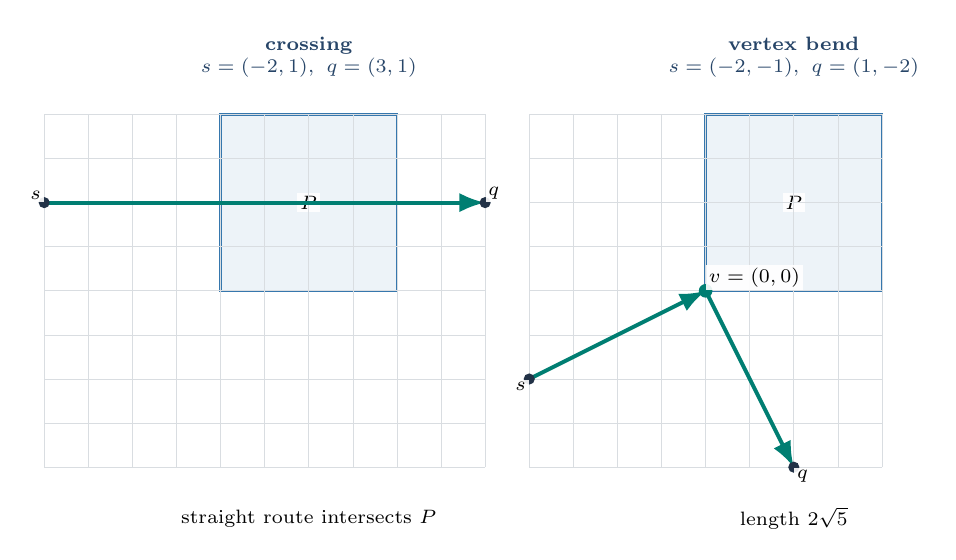
\begin{tikzpicture}[scale=1.12]
\begin{scope}
  \draw[polyA] (0,0) rectangle (2,2);
  \node[smalllabel] at (1,1) {\(P\)};
  \draw[coordgrid] (-2,-2) grid[step=.5] (3,2);
  \draw[route,-Latex] (-2,1)--(3,1);
  \fill[ink] (-2,1) circle (1.8pt); \fill[ink] (3,1) circle (1.8pt);
  \node[smalllabel,above left] at (-2,1) {\(s\)};
  \node[smalllabel,above right] at (3,1) {\(q\)};
  \node[font=\scriptsize\bfseries,color=navy,align=center] at (1,2.65)
    {crossing\\\(s=(-2,1),\ q=(3,1)\)};
  \node[smalllabel,align=center] at (1,-2.58)
    {straight route intersects \(P\)};
\end{scope}
\begin{scope}[xshift=5.5cm]
  \draw[polyA] (0,0) rectangle (2,2);
  \node[smalllabel] at (1,1) {\(P\)};
  \draw[coordgrid] (-2,-2) grid[step=.5] (2,2);
  \draw[route,-Latex] (-2,-1)--(0,0);
  \draw[route,-Latex] (0,0)--(1,-2);
  \fill[ink] (-2,-1) circle (1.8pt); \fill[ink] (1,-2) circle (1.8pt);
  \fill[good] (0,0) circle (2.2pt);
  \node[smalllabel,below left] at (-2,-1) {\(s\)};
  \node[smalllabel,below right] at (1,-2) {\(q\)};
  \node[smalllabel,above right] at (0,0) {\(v=(0,0)\)};
  \node[font=\scriptsize\bfseries,color=navy,align=center] at (1,2.65)
    {vertex bend\\\(s=(-2,-1),\ q=(1,-2)\)};
  \node[smalllabel] at (1,-2.58) {length \(2\sqrt5\)};
\end{scope}
\end{tikzpicture}}

\newcommand{\figrepeat}{%
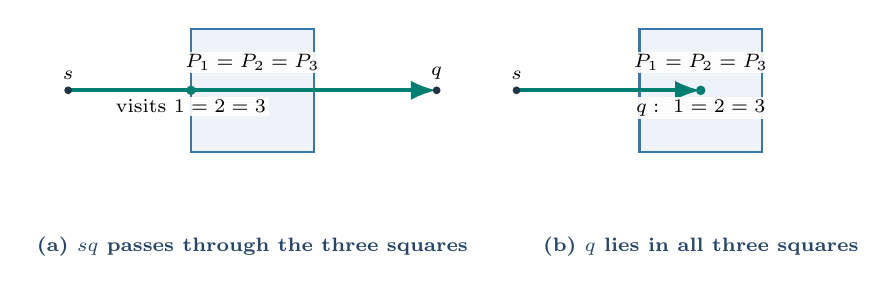
\begin{tikzpicture}[scale=.78]
\begin{scope}
\draw[polyA] (2,1) rectangle (4,3);
\node[smalllabel] at (3,2.45) {\(P_1=P_2=P_3\)};
\draw[route,-Latex] (0,2)--(6,2);
\fill[ink] (0,2) circle (1.8pt); \fill[ink] (6,2) circle (1.8pt);
\fill[good] (2,2) circle (2.2pt);
\node[smalllabel,above] at (0,2.12) {\(s\)};
\node[smalllabel,above] at (6,2.12) {\(q\)};
\node[smalllabel,below] at (2,1.9) {visits \(1=2=3\)};
\node[font=\scriptsize\bfseries,color=navy] at (3,-.55)
  {(a) \(sq\) passes through the three squares};
\end{scope}
\begin{scope}[xshift=7.3cm]
\draw[polyA] (2,1) rectangle (4,3);
\node[smalllabel] at (3,2.45) {\(P_1=P_2=P_3\)};
\draw[route,-Latex] (0,2)--(3,2);
\fill[ink] (0,2) circle (1.8pt); \fill[good] (3,2) circle (2.2pt);
\node[smalllabel,above] at (0,2.12) {\(s\)};
\node[smalllabel,below] at (3,1.9) {\(q:\ 1=2=3\)};
\node[font=\scriptsize\bfseries,color=navy] at (3,-.55)
  {(b) \(q\) lies in all three squares};
\end{scope}
\end{tikzpicture}}

\newcommand{\figfalsecrossing}{%
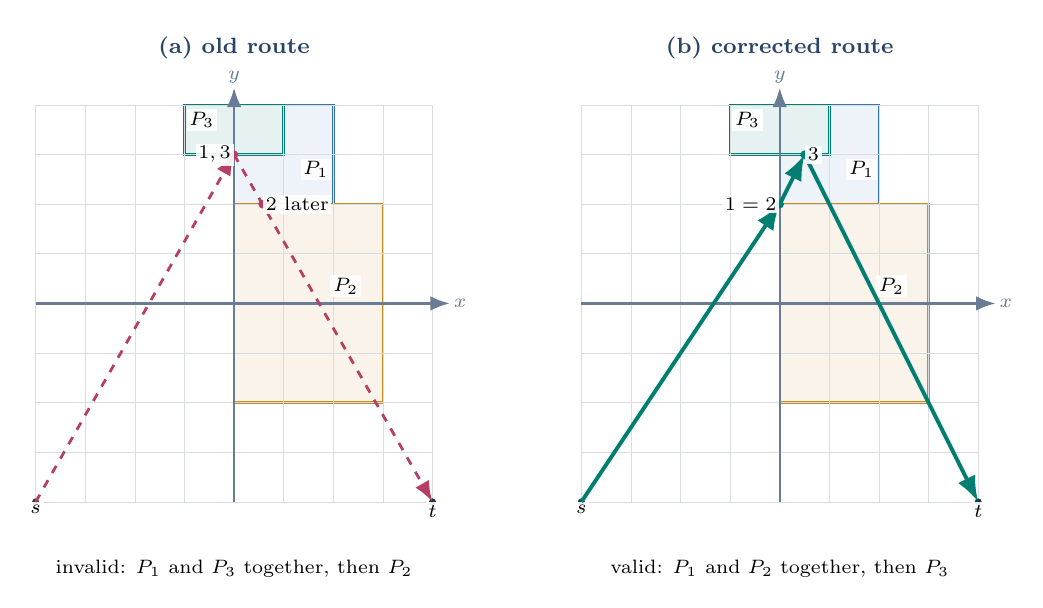
\begin{tikzpicture}[scale=.63]
\begin{scope}
  \draw[polyA] (0,2) rectangle (2,4);
  \draw[polyB] (0,-2) rectangle (3,2);
  \draw[draw=good,fill=good!10,line width=.9pt] (-1,3) rectangle (1,4);
  \draw[coordgrid] (-4,-4) grid[step=1] (4,4);
  \draw[navy!70,-Latex,line width=.9pt] (-4,0)--(4.35,0)
    node[smalllabel,right] {\(x\)};
  \draw[navy!70,-Latex,line width=.9pt] (0,-4)--(0,4.35)
    node[smalllabel,above] {\(y\)};
  \node[smalllabel] at (1.65,2.7) {\(P_1\)};
  \node[smalllabel] at (2.25,.35) {\(P_2\)};
  \node[smalllabel] at (-.65,3.7) {\(P_3\)};
  \fill[ink] (-4,-4) circle (2pt); \fill[ink] (4,-4) circle (2pt);
  \node[smalllabel,below] at (-4,-4) {\(s\)};
  \node[smalllabel,below] at (4,-4) {\(t\)};
  \draw[wrong,-Latex] (-4,-4)--(0,3);
  \draw[wrong,-Latex] (0,3)--(4,-4);
  \fill[bad] (0,3) circle (2.4pt);
  \fill[bad] (4/7,2) circle (2.4pt);
  \node[smalllabel,left] at (0,3) {\(1,3\)};
  \node[smalllabel,right] at (4/7,2) {\(2\) later};
  \node[smalllabel,align=center] at (0,-5.35)
    {invalid: \(P_1\) and \(P_3\) together, then \(P_2\)};
  \node[font=\footnotesize\bfseries,color=navy] at (0,5.15) {(a) old route};
\end{scope}
\begin{scope}[xshift=11cm]
  \draw[polyA] (0,2) rectangle (2,4);
  \draw[polyB] (0,-2) rectangle (3,2);
  \draw[draw=good,fill=good!10,line width=.9pt] (-1,3) rectangle (1,4);
  \draw[coordgrid] (-4,-4) grid[step=1] (4,4);
  \draw[navy!70,-Latex,line width=.9pt] (-4,0)--(4.35,0)
    node[smalllabel,right] {\(x\)};
  \draw[navy!70,-Latex,line width=.9pt] (0,-4)--(0,4.35)
    node[smalllabel,above] {\(y\)};
  \node[smalllabel] at (1.65,2.7) {\(P_1\)};
  \node[smalllabel] at (2.25,.35) {\(P_2\)};
  \node[smalllabel] at (-.65,3.7) {\(P_3\)};
  \fill[ink] (-4,-4) circle (2pt); \fill[ink] (4,-4) circle (2pt);
  \node[smalllabel,below] at (-4,-4) {\(s\)};
  \node[smalllabel,below] at (4,-4) {\(t\)};
  \draw[route,-Latex] (-4,-4)--(0,2);
  \draw[route,-Latex] (0,2)--(.5,3);
  \draw[route,-Latex] (.5,3)--(4,-4);
  \fill[good] (0,2) circle (2.4pt); \fill[good] (.5,3) circle (2.4pt);
  \node[smalllabel,left] at (0,2) {\(1=2\)};
  \node[smalllabel,right] at (.5,3) {\(3\)};
  \node[smalllabel,align=center] at (0,-5.35)
    {valid: \(P_1\) and \(P_2\) together, then \(P_3\)};
  \node[font=\footnotesize\bfseries,color=navy] at (0,5.15) {(b) corrected route};
\end{scope}
\end{tikzpicture}}

\newcommand{\figfalsecrossingzoom}{%
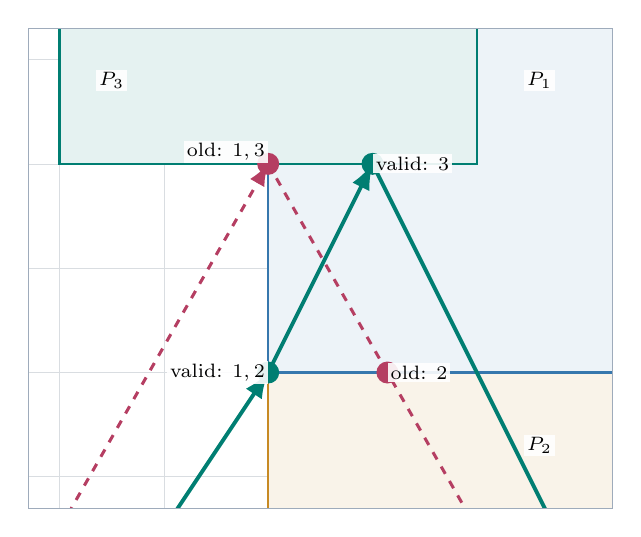
\begin{tikzpicture}[scale=2.65]
\begin{scope}
  \clip (-1.15,1.35) rectangle (1.65,3.65);
  \draw[coordgrid] (-2,1) grid[step=.5] (2,4);
  \draw[polyB] (0,-2) rectangle (3,2);
  \draw[polyA] (0,2) rectangle (2,4);
  \draw[draw=good,fill=good!10,line width=.9pt] (-1,3) rectangle (1,4);
  \draw[wrong,-Latex,line width=1.1pt] (-4,-4)--(0,3);
  \draw[wrong,-Latex,line width=1.1pt] (0,3)--(4,-4);
  \draw[route,-Latex] (-4,-4)--(0,2);
  \draw[route,-Latex] (0,2)--(.5,3);
  \draw[route,-Latex] (.5,3)--(4,-4);
\end{scope}
\draw[navy!45] (-1.15,1.35) rectangle (1.65,3.65);
\fill[bad] (0,3) circle (1.5pt); \fill[bad] (4/7,2) circle (1.5pt);
\fill[good] (0,2) circle (1.5pt); \fill[good] (.5,3) circle (1.5pt);
\node[smalllabel,above left] at (0,3) {old: \(1,3\)};
\node[smalllabel,right] at (4/7,2) {old: \(2\)};
\node[smalllabel,left] at (0,2) {valid: \(1,2\)};
\node[smalllabel,right] at (.5,3) {valid: \(3\)};
\node[smalllabel] at (-.75,3.4) {\(P_3\)};
\node[smalllabel] at (1.3,3.4) {\(P_1\)};
\node[smalllabel] at (1.3,1.65) {\(P_2\)};
\end{tikzpicture}}

\newcommand{\figordered}{%
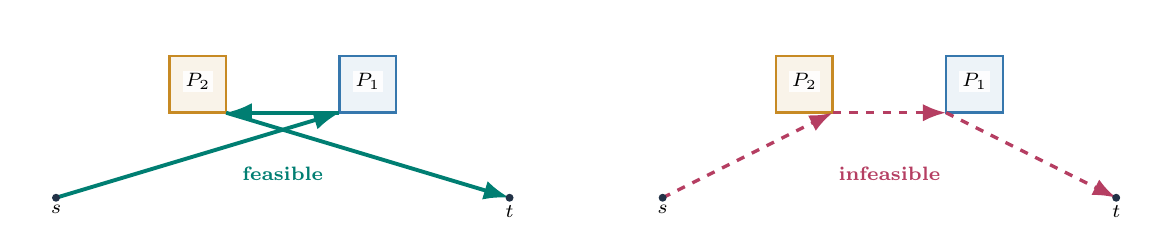
\begin{tikzpicture}[scale=.72]
\begin{scope}
  \path (-.5,-.45) rectangle (8.5,3);
  \draw[polyB] (2,1.5) rectangle (3,2.5);
  \draw[polyA] (5,1.5) rectangle (6,2.5);
  \node[smalllabel] at (2.5,2.05) {\(P_2\)};
  \node[smalllabel] at (5.5,2.05) {\(P_1\)};
  \draw[route,-Latex] (0,0)--(5,1.5);
  \draw[route,-Latex] (5,1.5)--(3,1.5);
  \draw[route,-Latex] (3,1.5)--(8,0);
  \foreach \x/\y/\lab in {0/0/s,8/0/t}
    {\fill[ink] (\x,\y) circle (2pt);
     \node[smalllabel,below] at (\x,\y-.08) {\(\lab\)};}
  \node[font=\scriptsize\bfseries,color=good] at (4,.42) {feasible};
\end{scope}
\begin{scope}[xshift=10.7cm]
  \path (-.5,-.45) rectangle (8.5,3);
  \draw[polyB] (2,1.5) rectangle (3,2.5);
  \draw[polyA] (5,1.5) rectangle (6,2.5);
  \node[smalllabel] at (2.5,2.05) {\(P_2\)};
  \node[smalllabel] at (5.5,2.05) {\(P_1\)};
  \draw[wrong,-Latex,line width=1.2pt] (0,0)--(3,1.5);
  \draw[wrong,-Latex,line width=1.2pt] (3,1.5)--(5,1.5);
  \draw[wrong,-Latex,line width=1.2pt] (5,1.5)--(8,0);
  \foreach \x/\y/\lab in {0/0/s,8/0/t}
    {\fill[ink] (\x,\y) circle (2pt);
     \node[smalllabel,below] at (\x,\y-.08) {\(\lab\)};}
  \node[font=\scriptsize\bfseries,color=bad] at (4,.42) {infeasible};
\end{scope}
\end{tikzpicture}}
\newcommand{\figcontacts}{%
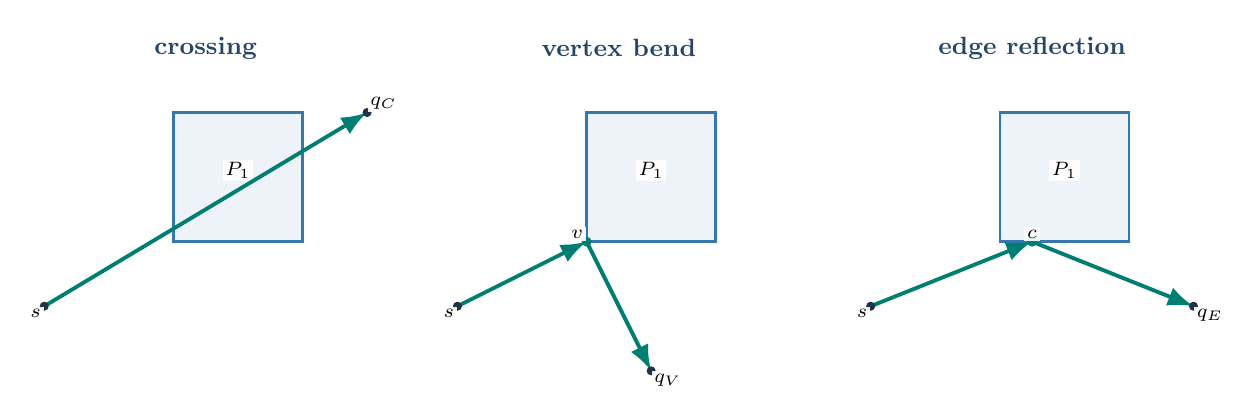
\begin{tikzpicture}[scale=.82]
\begin{scope}
  \draw[polyA] (0,0) rectangle (2,2);
  \node[smalllabel] at (1,1.1) {\(P_1\)};
  \draw[route,-Latex] (-2,-1)--(3,2);
  \fill[ink] (-2,-1) circle (2pt); \fill[ink] (3,2) circle (2pt);
  \node[smalllabel,below left] at (-2,-1) {\(s\)};
  \node[smalllabel,above right] at (3,2) {\(q_C\)};
  \node[font=\small\bfseries,color=navy] at (.5,3) {crossing};
\end{scope}
\begin{scope}[xshift=6.4cm]
  \draw[polyA] (0,0) rectangle (2,2);
  \node[smalllabel] at (1,1.1) {\(P_1\)};
  \draw[route,-Latex] (-2,-1)--(0,0);
  \draw[route,-Latex] (0,0)--(1,-2);
  \fill[ink] (-2,-1) circle (2pt); \fill[ink] (1,-2) circle (2pt);
  \fill[good] (0,0) circle (2.2pt);
  \node[smalllabel,below left] at (-2,-1) {\(s\)};
  \node[smalllabel,below right] at (1,-2) {\(q_V\)};
  \node[smalllabel,above left] at (0,0) {\(v\)};
  \node[font=\small\bfseries,color=navy] at (.5,3) {vertex bend};
\end{scope}
\begin{scope}[xshift=12.8cm]
  \draw[polyA] (0,0) rectangle (2,2);
  \node[smalllabel] at (1,1.1) {\(P_1\)};
  \draw[route,-Latex] (-2,-1)--(.5,0);
  \draw[route,-Latex] (.5,0)--(3,-1);
  \fill[ink] (-2,-1) circle (2pt); \fill[ink] (3,-1) circle (2pt);
  \fill[good] (.5,0) circle (2.2pt);
  \node[smalllabel,below left] at (-2,-1) {\(s\)};
  \node[smalllabel,below right] at (3,-1) {\(q_E\)};
  \node[smalllabel,above] at (.5,0) {\(c\)};
  \node[font=\small\bfseries,color=navy] at (.5,3) {edge reflection};
\end{scope}
\end{tikzpicture}}
\newcommand{\figunfold}{%
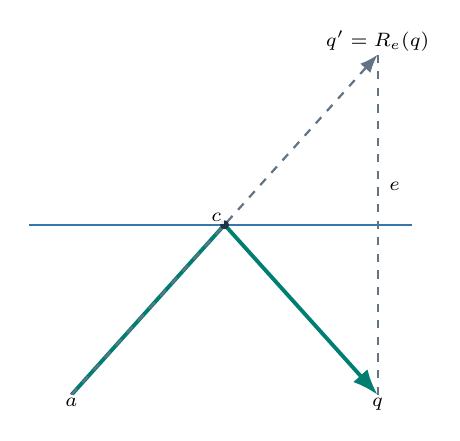
\begin{tikzpicture}[scale=1.08]
\draw[polyA] (-.3,0)--(4.2,0); \node[smalllabel] at (4, .45) {\(e\)};
\coordinate (S) at (.2,-2); \coordinate (C) at (2,0); \coordinate (Q) at (3.8,-2); \coordinate (R) at (3.8,2);
\draw[route,-Latex] (S)--(C)--(Q); \draw[aux,-Latex] (S)--(R);
\draw[aux] (Q)--(R); \fill[ink] (C) circle (1.5pt);
\node[smalllabel,below] at (S) {\(a\)}; \node[smalllabel,below] at (Q) {\(q\)};
\node[smalllabel,above] at (R) {\(q'=R_e(q)\)};
\node[smalllabel,above left] at (C) {\(c\)};
\end{tikzpicture}}
\newcommand{\figlastmap}{%
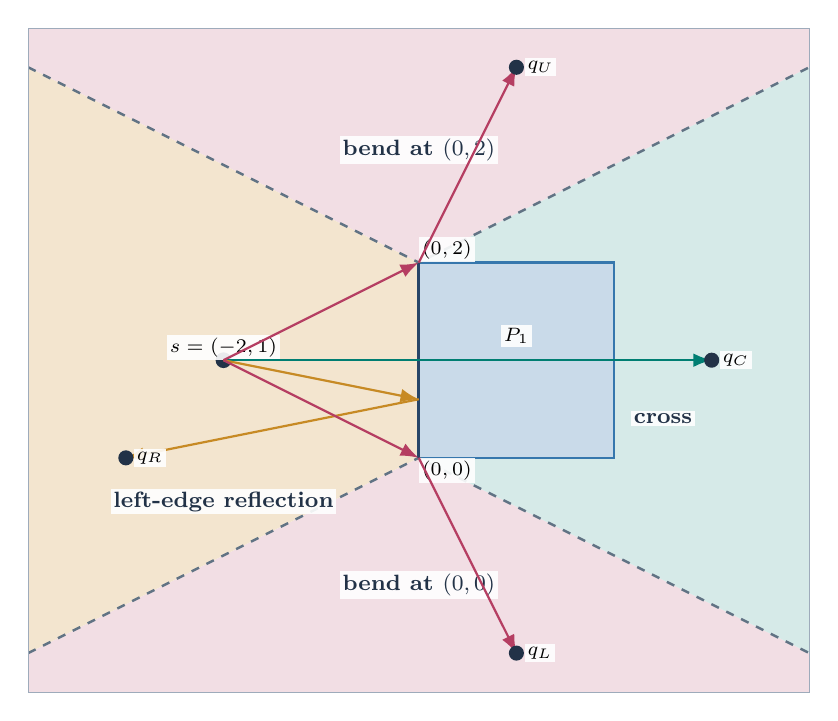
\begin{tikzpicture}[scale=1.24]
\begin{scope}
  \clip (-4,-2.4) rectangle (4,4.4);
  \fill[bad!17] (-4,-2.4)--(4,-2.4)--(4,-2)--(0,0)--(-4,-2)--cycle;
  \fill[bad!17] (-4,4.4)--(4,4.4)--(4,4)--(0,2)--(-4,4)--cycle;
  \fill[pTwo!22] (-4,-2)--(0,0)--(0,2)--(-4,4)--cycle;
  \fill[good!16] (0,0)--(4,-2)--(4,4)--(0,2)--cycle;
  \draw[polyA,fill=pOne!27] (0,0) rectangle (2,2);
  \draw[aux,line width=.9pt] (-4,-2)--(0,0)--(4,-2);
  \draw[aux,line width=.9pt] (-4,4)--(0,2)--(4,4);
  \draw[very thick,navy] (0,0)--(0,2);
\end{scope}
\draw[navy!45] (-4,-2.4) rectangle (4,4.4);
\fill[ink] (-2,1) circle (2.3pt);
\node[smalllabel,above] at (-2,1) {\(s=(-2,1)\)};
\node[smalllabel] at (1,1.25) {\(P_1\)};
\node[smalllabel,font=\footnotesize\bfseries,text=ink] at (0,3.15) {bend at \((0,2)\)};
\node[smalllabel,font=\footnotesize\bfseries,text=ink] at (0,-1.3) {bend at \((0,0)\)};
\node[smalllabel,font=\footnotesize\bfseries,text=ink] at (-2,-.45) {left-edge reflection};
\node[smalllabel,font=\footnotesize\bfseries,text=ink] at (2.5,.4) {cross};
\node[smalllabel,below right] at (0,0) {\((0,0)\)};
\node[smalllabel,above right] at (0,2) {\((0,2)\)};
\draw[good,-Latex,line width=.8pt] (-2,1)--(3,1);
\draw[pTwo,-Latex,line width=.8pt] (-2,1)--(0,.6);
\draw[pTwo,-Latex,line width=.8pt] (0,.6)--(-3,0);
\draw[bad,-Latex,line width=.8pt] (-2,1)--(0,2);
\draw[bad,-Latex,line width=.8pt] (0,2)--(1,4);
\draw[bad,-Latex,line width=.8pt] (-2,1)--(0,0);
\draw[bad,-Latex,line width=.8pt] (0,0)--(1,-2);
\foreach \x/\y/\lab in {3/1/C,-3/0/R,1/4/U,1/-2/L}
  {\fill[ink] (\x,\y) circle (2.2pt);
   \node[smalllabel,right] at (\x+.08,\y) {\(q_{\lab}\)};}
\end{tikzpicture}}

\newcommand{\figwitnesssetup}{%
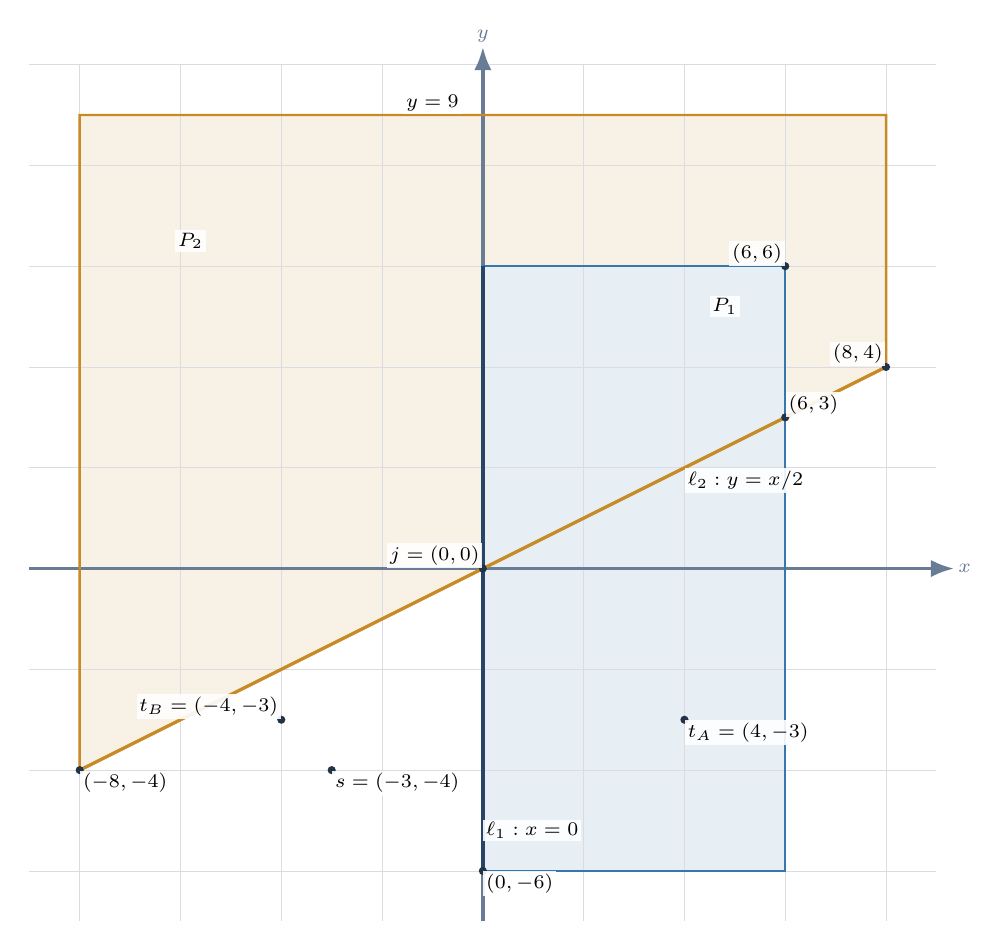
\begin{tikzpicture}[scale=.64]
  \path[fill=pTwo!12] (-8,-4)--(8,4)--(8,9)--(-8,9)--cycle;
  \path[fill=pOne!12] (0,-6) rectangle (6,6);
  \draw[coordgrid] (-9,-7) grid[step=2] (9,10);
  \draw[navy!70,-Latex,line width=1.2pt] (-9,0)--(9.35,0)
    node[smalllabel,right] {\(x\)};
  \draw[navy!70,-Latex,line width=1.2pt] (0,-7)--(0,10.35)
    node[smalllabel,above] {\(y\)};
  \draw[polyB,fill=none] (-8,-4)--(8,4)--(8,9)--(-8,9)--cycle;
  \draw[polyA,fill=none] (0,-6) rectangle (6,6);
  \draw[very thick,navy] (0,-6)--(0,6);
  \draw[very thick,pTwo] (-8,-4)--(8,4);
  \node[smalllabel] at (4.8,5.2) {\(P_1\)};
  \node[smalllabel] at (-5.8,6.5) {\(P_2\)};
  \foreach \x/\y in {-3/-4,0/0,4/-3,-4/-3,6/3}
    {\fill[ink] (\x,\y) circle (2.3pt);}
  \foreach \x/\y in {0/-6,6/6,-8/-4,8/4}
    {\fill[ink] (\x,\y) circle (2.3pt);}
  \node[smalllabel,below right] at (-3,-4) {\(s=(-3,-4)\)};
  \node[smalllabel,above left] at (-4,-3) {\(t_B=(-4,-3)\)};
  \node[smalllabel,below right] at (4,-3) {\(t_A=(4,-3)\)};
  \node[smalllabel,above left] at (0,0) {\(j=(0,0)\)};
  \node[smalllabel,above right] at (6,3) {\((6,3)\)};
  \node[smalllabel,below right] at (0,-6) {\((0,-6)\)};
  \node[smalllabel,above left] at (6,6) {\((6,6)\)};
  \node[smalllabel,below right] at (-8,-4) {\((-8,-4)\)};
  \node[smalllabel,above left] at (8,4) {\((8,4)\)};
  \node[smalllabel,above] at (-1,9) {\(y=9\)};
  \node[smalllabel,right] at (0,-5.2) {\(\ell_1:x=0\)};
  \node[smalllabel,below right] at (4,2) {\(\ell_2:y=x/2\)};
\end{tikzpicture}}
\newcommand{\figbinary}{%
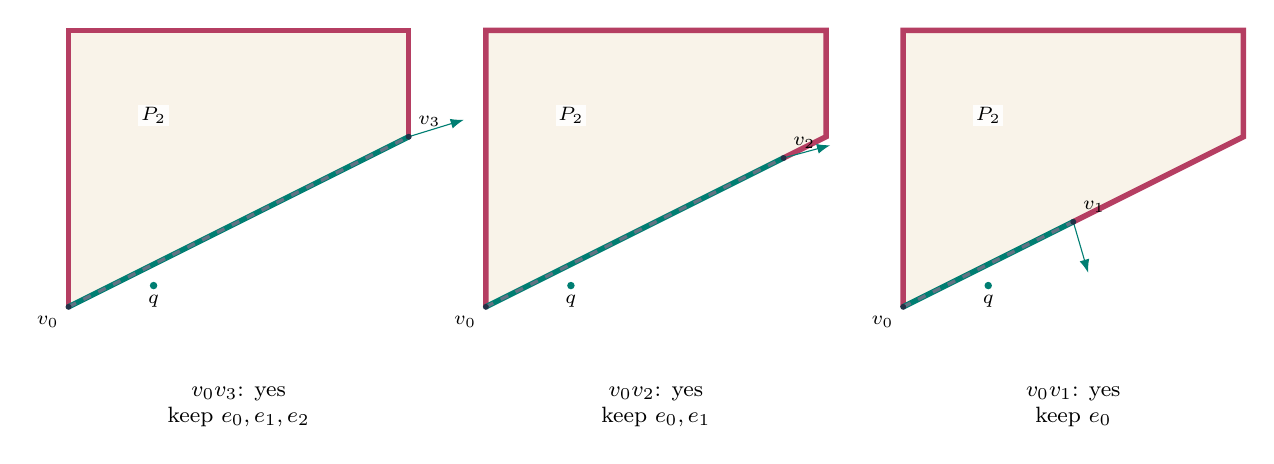
\begin{tikzpicture}
\foreach \shift/\j/\endx/\endy/\rayx/\rayy/\txt in
 {0/3/8/4/2.6/.8/{keep \(e_0,e_1,e_2\)},
  5.3/2/6/3/2.2/.6/{keep \(e_0,e_1\)},
  10.6/1/0/0/.7/-2.4/{keep \(e_0\)}} {
  \begin{scope}[xshift=\shift cm,scale=.27]
    \draw[polyB] (-8,-4)--(0,0)--(6,3)--(8,4)--(8,9)--(-8,9)--cycle;
    \node[smalllabel] at (-4,5) {\(P_2\)};
    \draw[bad,line width=2pt] (\endx,\endy)--(8,4)--(8,9)--(-8,9)--(-8,-4);
    \draw[good,line width=2pt] (-8,-4)--(\endx,\endy);
    \draw[aux,line width=1.2pt] (-8,-4)--(\endx,\endy);
    \draw[good,-Latex] (\endx,\endy)--++(\rayx,\rayy);
    \fill[ink] (-8,-4) circle (4pt);
    \fill[ink] (\endx,\endy) circle (4pt);
    \fill[good] (-4,-3) circle (5pt);
    \node[font=\scriptsize,below left] at (-8,-4) {\(v_0\)};
    \node[font=\scriptsize,above right] at (\endx,\endy) {\(v_{\j}\)};
    \node[font=\scriptsize,below] at (-4,-3) {\(q\)};
  \end{scope}
  \node[font=\footnotesize,align=center] at (\shift cm,-2.35cm)
    {\(v_0v_{\j}\): yes\\\txt};
}
\end{tikzpicture}}
\newcommand{\figsplit}{%
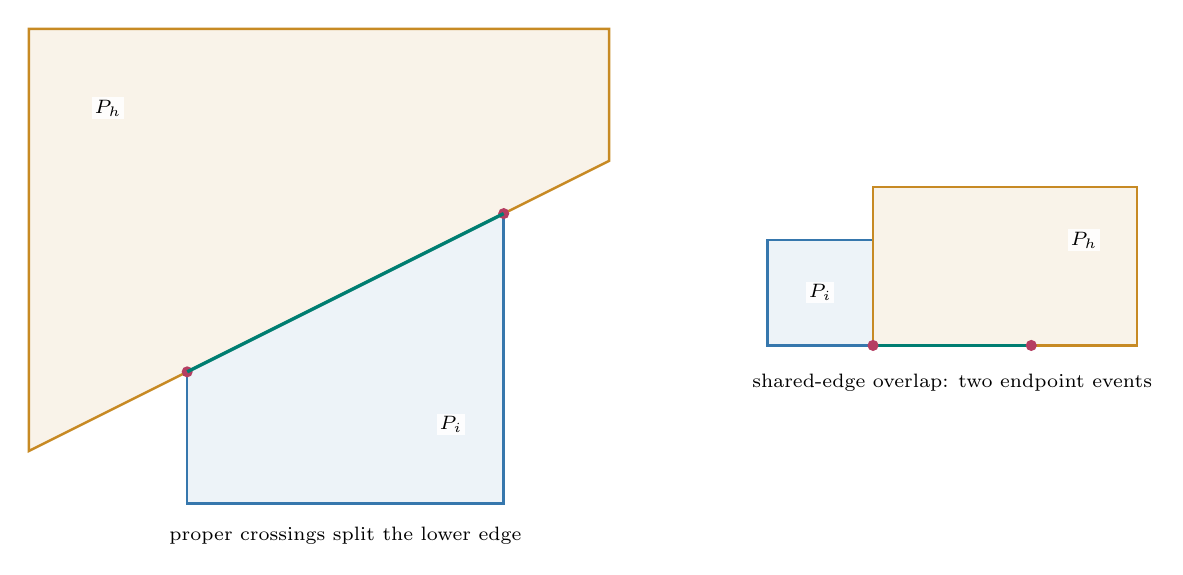
\begin{tikzpicture}[scale=.67]
\draw[polyA] (0,-3) rectangle (6,4);
\draw[polyB] (-3,-2)--(8,3.5)--(8,6)--(-3,6)--cycle;
\node[smalllabel] at (5,-1.5) {\(P_i\)};
\node[smalllabel] at (-1.5,4.5) {\(P_h\)};
\foreach \x/\y in {0/-.5,6/2.5} {\fill[bad] (\x,\y) circle (3pt);}
\draw[very thick,good] (0,-.5)--(6,2.5);
\node[smalllabel] at (3,-3.6) {proper crossings split the lower edge};
\begin{scope}[xshift=11cm]
\draw[polyA] (0,0) rectangle (5,2);
\draw[polyB] (2,0) rectangle (7,3);
\node[smalllabel] at (1,1) {\(P_i\)};
\node[smalllabel] at (6,2) {\(P_h\)};
\draw[very thick,good] (2,0)--(5,0);
\fill[bad] (2,0) circle (3pt); \fill[bad] (5,0) circle (3pt);
\node[smalllabel] at (3.5,-.7) {shared-edge overlap: two endpoint events};
\end{scope}
\end{tikzpicture}}
\newcommand{\figlimits}{%
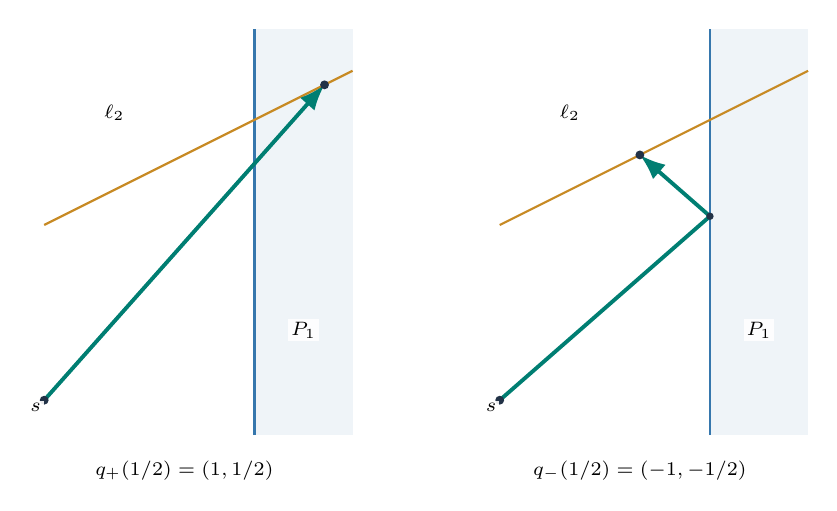
\begin{tikzpicture}[scale=.89]
\begin{scope}
\fill[pOne!8] (0,-4.5) rectangle (1.4,1.3);\draw[pOne,thick] (0,-4.5)--(0,1.3);
\draw[pTwo,thick] (-3,-1.5)--(1.4,.7);\draw[route,-Latex] (-3,-4)--(1,.5);
\node[smalllabel] at (.7,-3) {\(P_1\)};
\node[smalllabel] at (-2,.1) {\(\ell_2\)};
\fill[ink] (-3,-4) circle (1.8pt); \fill[ink] (1,.5) circle (1.8pt);
\node[smalllabel,below left] at (-3,-4) {\(s\)};
\node[smalllabel] at (-1,-5) {\(q_+(1/2)=(1,1/2)\)};
\end{scope}
\begin{scope}[xshift=6.5cm]
\fill[pOne!8] (0,-4.5) rectangle (1.4,1.3);\draw[pOne,thick] (0,-4.5)--(0,1.3);
\draw[pTwo,thick] (-3,-1.5)--(1.4,.7);\draw[route,-Latex] (-3,-4)--(0,-11/8)--(-1,-.5);
\node[smalllabel] at (.7,-3) {\(P_1\)};
\node[smalllabel] at (-2,.1) {\(\ell_2\)};
\fill[ink] (-3,-4) circle (1.8pt); \fill[ink] (-1,-.5) circle (1.8pt);
\node[smalllabel,below left] at (-3,-4) {\(s\)};
\fill[ink] (0,-11/8) circle (1.5pt);
\node[smalllabel] at (-1,-5) {\(q_-(1/2)=(-1,-1/2)\)};
\end{scope}
\end{tikzpicture}}
\newcommand{\figrays}{%
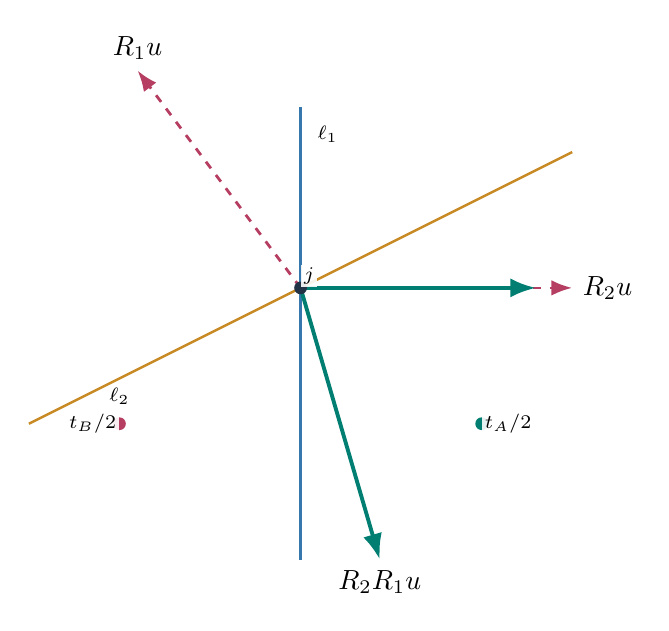
\begin{tikzpicture}[scale=1.15]
\coordinate (J) at (0,0);
\draw[polyA] (0,-3)--(0,2); \draw[polyB] (-3,-1.5)--(3,1.5);
\node[smalllabel] at (.3,1.7) {\(\ell_1\)};
\node[smalllabel] at (-2,-1.2) {\(\ell_2\)};
\draw[wrong,-Latex] (J)--(-1.8,2.4) node[above] {\(R_1u\)};
\draw[wrong,-Latex] (J)--(3,0) node[right] {\(R_2u\)};
\draw[route,-Latex] (J)--(.875,-3) node[below] {\(R_2R_1u\)};
\draw[route,-Latex] (J)--(2.6,0);
\fill[ink] (J) circle (2pt);\node[smalllabel,above right] at (J) {\(j\)};
\fill[good] (2,-1.5) circle (2pt);\node[smalllabel,right] at (2,-1.5) {\(t_A/2\)};
\fill[bad] (-2,-1.5) circle (2pt);\node[smalllabel,left] at (-2,-1.5) {\(t_B/2\)};
\end{tikzpicture}}
\newcommand{\figvirtual}{%
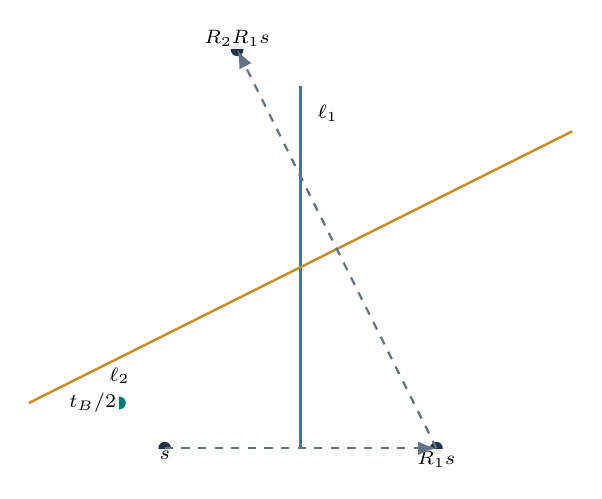
\begin{tikzpicture}[scale=1.15]
\draw[polyA] (0,-2)--(0,2);\draw[polyB] (-3,-1.5)--(3,1.5);
\node[smalllabel] at (.3,1.7) {\(\ell_1\)};
\node[smalllabel] at (-2,-1.2) {\(\ell_2\)};
\coordinate (S) at (-1.5,-2);\coordinate (V1) at (1.5,-2);\coordinate (V2) at (-.7,2.4);
\fill[ink] (S) circle (2pt);\fill[ink] (V1) circle (2pt);\fill[ink] (V2) circle (2pt);
\node[smalllabel,below] at (S) {\(s\)};\node[smalllabel,below] at (V1) {\(R_1s\)};
\node[smalllabel,above] at (V2) {\(R_2R_1s\)};
\draw[aux,-Latex] (S)--(V1);\draw[aux,-Latex] (V1)--(V2);
\fill[good] (-2,-1.5) circle (2pt);\node[smalllabel,left] at (-2,-1.5) {\(t_B/2\)};
\end{tikzpicture}}
\newcommand{\figpath}{%
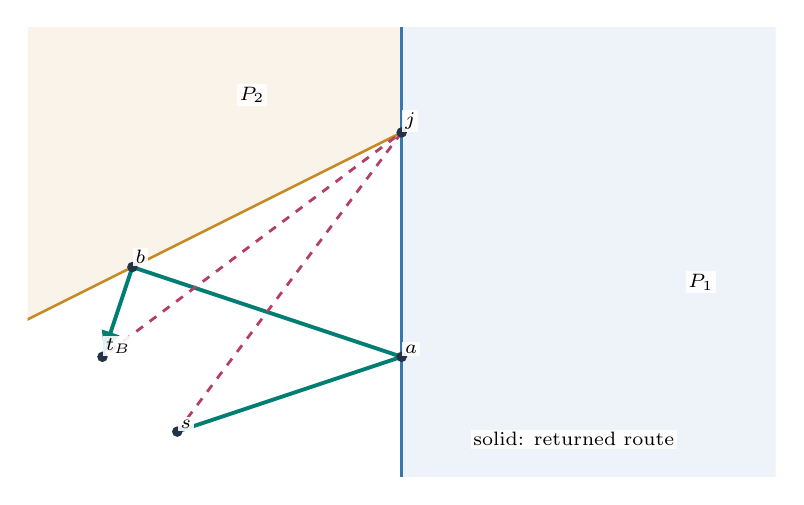
\begin{tikzpicture}[scale=.95]
\begin{scope}
\clip (-5,-4.6) rectangle (5,1.4);
\draw[polyB] (-8,-4)--(8,4)--(8,9)--(-8,9)--cycle;
\draw[polyA] (0,-6) rectangle (6,6);
\node[smalllabel] at (4,-2) {\(P_1\)};
\node[smalllabel] at (-2,.5) {\(P_2\)};
\draw[route,-Latex] (-3,-4)--(0,-3)--(-3.6,-1.8)--(-4,-3);
\draw[wrong] (-3,-4)--(0,0)--(-4,-3);
\end{scope}
\foreach \x/\y/\lab in {-3/-4/s,0/-3/a,-3.6/-1.8/b,-4/-3/t_B,0/0/j}
  {\fill[ink] (\x,\y) circle (2pt);\node[smalllabel,above right] at (\x,\y) {\(\lab\)};}
\node[smalllabel] at (2.3,-4.1) {solid: returned route};
\end{tikzpicture}}
\newcommand{\figbackwards}{%
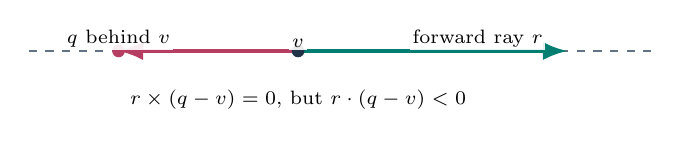
\begin{tikzpicture}[scale=1.14]
\draw[aux] (-3,0)--(4,0);
\draw[good,-Latex,line width=1.3pt] (0,0)--(3,0);
\draw[bad,-Latex,line width=1.3pt] (0,0)--(-2,0);
\fill[ink] (0,0) circle (2pt); \fill[bad] (-2,0) circle (2pt);
\node[smalllabel,above] at (0,0) {\(v\)};
\node[smalllabel,above] at (2,0) {forward ray \(r\)};
\node[smalllabel,above] at (-2,0) {\(q\) behind \(v\)};
\node[smalllabel,below] at (0,-.4) {\(r\times(q-v)=0\), but \(r\cdot(q-v)<0\)};
\end{tikzpicture}}
\newcommand{\figmembership}{%
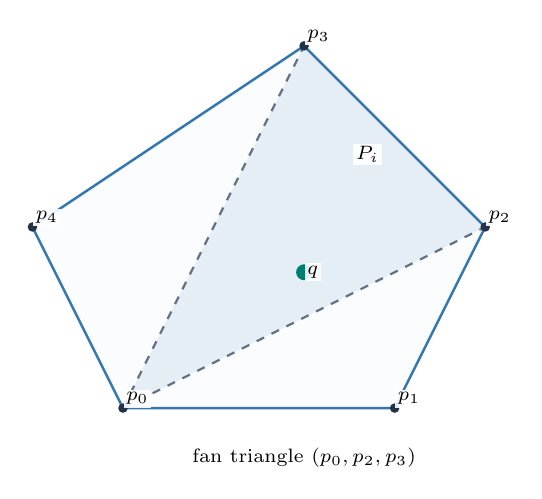
\begin{tikzpicture}[scale=1.15]
\fill[pOne!14] (0,0)--(4,2)--(2,4)--cycle;
\draw[polyA,fill opacity=.25] (0,0)--(3,0)--(4,2)--(2,4)--(-1,2)--cycle;
\node[smalllabel] at (2.7,2.8) {\(P_i\)};
\draw[aux] (0,0)--(4,2); \draw[aux] (0,0)--(2,4);
\fill[good] (2,1.5) circle (2.5pt);
\foreach \x/\y/\n in {0/0/0,3/0/1,4/2/2,2/4/3,-1/2/4}
  {\fill[ink] (\x,\y) circle (1.5pt);\node[smalllabel,above right] at (\x,\y) {\(p_{\n}\)};}
\node[smalllabel,right] at (2,1.5) {\(q\)};
\node[smalllabel] at (2,-.55) {fan triangle \((p_0,p_2,p_3)\)};
\end{tikzpicture}}

% A sign decision is a coefficient comparison, not a numerically tiny offset.
\newcommand{\figsymbolic}{%
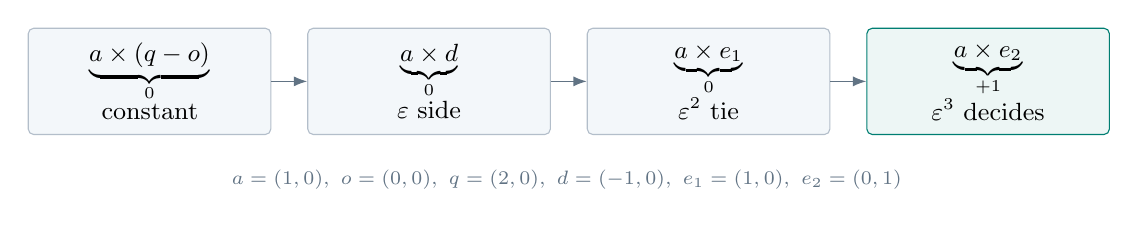
\begin{tikzpicture}[font=\small,
 stage/.style={draw=navy!35,fill=codebg,rounded corners=2pt,
                 text width=2.8cm,minimum height=1.35cm,align=center,inner sep=4pt}]
\node[stage] (a) at (0,0) {\(\underbrace{a\times(q-o)}_{0}\)\\constant};
\node[stage] (b) at (3.55,0) {\(\underbrace{a\times d}_{0}\)\\\(\varepsilon\) side};
\node[stage] (c) at (7.1,0) {\(\underbrace{a\times e_1}_{0}\)\\\(\varepsilon^2\) tie};
\node[stage,draw=good,fill=good!7] (d) at (10.65,0)
  {\(\underbrace{a\times e_2}_{+1}\)\\\(\varepsilon^3\) decides};
\foreach \u/\v in {a/b,b/c,c/d} \draw[quiet,-Latex] (\u.east)--(\v.west);
\node[font=\scriptsize,color=quiet,align=center] at (5.3,-1.25)
  {\(a=(1,0),\ o=(0,0),\ q=(2,0),\ d=(-1,0),\ e_1=(1,0),\ e_2=(0,1)\)};
\end{tikzpicture}}

% Two rows distinguish recursive query transforms from physical refolding.
\newcommand{\figrefoldtrace}{%
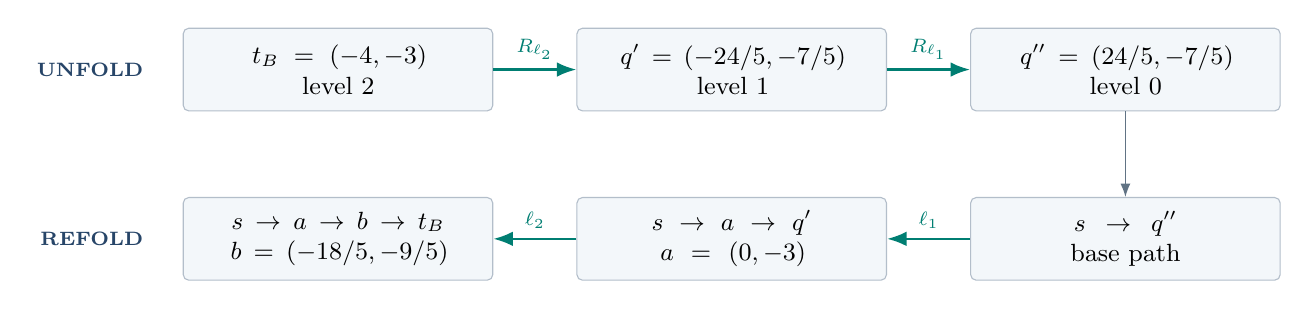
\begin{tikzpicture}[font=\small,
 tracebox/.style={draw=navy!35,fill=codebg,rounded corners=2pt,
              text width=3.65cm,minimum height=1.05cm,align=center,inner sep=4pt}]
\node[font=\scriptsize\bfseries,color=navy,anchor=east] at (-.35,0)
  {UNFOLD};
\node[tracebox] (q) at (2,0) {\(t_B=(-4,-3)\)\\level 2};
\node[tracebox] (qp) at (7,0) {\(q'=(-24/5,-7/5)\)\\level 1};
\node[tracebox] (qpp) at (12,0) {\(q''=(24/5,-7/5)\)\\level 0};
\draw[good,-Latex,line width=.9pt] (q.east)--node[above,font=\scriptsize]{\(R_{\ell_2}\)}(qp.west);
\draw[good,-Latex,line width=.9pt] (qp.east)--node[above,font=\scriptsize]{\(R_{\ell_1}\)}(qpp.west);
\node[font=\scriptsize\bfseries,color=navy,anchor=east] at (-.35,-2.15)
  {REFOLD};
\node[tracebox] (p2) at (2,-2.15) {\(s\to a\to b\to t_B\)\\\(b=(-18/5,-9/5)\)};
\node[tracebox] (p1) at (7,-2.15) {\(s\to a\to q'\)\\\(a=(0,-3)\)};
\node[tracebox] (p0) at (12,-2.15) {\(s\to q''\)\\base path};
\draw[good,-Latex,line width=.9pt] (p0.west)--node[above,font=\scriptsize]{\(\ell_1\)}(p1.east);
\draw[good,-Latex,line width=.9pt] (p1.west)--node[above,font=\scriptsize]{\(\ell_2\)}(p2.east);
\draw[quiet,-Latex] (qpp.south)--(p0.north);
\end{tikzpicture}}

\begin{document}
\begin{titlepage}
\thispagestyle{empty}
{\sffamily\small\bfseries\color{good}GEOMETRY \quad\textbullet\quad ALGORITHM \quad\textbullet\quad C++ SOURCE}\par
\vspace{12mm}
{\fontsize{28}{33}\selectfont\bfseries\color{navy}Fixed-order convex\par
polygon tours}\par
\vspace{4mm}
{\Large From contact geometry to directional last-step maps}\par
\vspace{4mm}
{\large\color{quiet}A visual guide to the current implementation and its exact counterexample}\par
\vspace{15mm}
\begin{center}\resizebox{.86\textwidth}{!}{\figpath}\end{center}
\vspace{5mm}
\begin{coverbox}
\textbf{What this guide does.} It derives the three last-step actions, shows why intersection vertices need one-sided information, and walks through symbolic queries, virtual sources, binary location, and refolding in the current C++ solver. The exact two-target witness is independently certified. The remaining general proof obligation for closed degeneracies is kept explicit.
\end{coverbox}
\vfill
{\small\color{quiet}TouringPolygons source revision \code{0aaf550} \quad / \quad 14 September 2026}\par
\end{titlepage}
{\sffamily\scriptsize\bfseries\color{good}READING MAP \hfill 14 SECTIONS \quad\textbullet\quad 12 FIGURES}\par
\vspace{2mm}
{\color{navy!25}\hrule height .5pt}
\vspace{5mm}
\begingroup\setlength{\parskip}{0pt}\tableofcontents\thispagestyle{fancy}\endgroup
\vspace{7mm}
\begin{sourcebox}
\raggedright
\textbf{Code key.} Line numbers refer to source revision \code{0aaf550}. For IM, BS, SOL, and VAL, prepend \path{packages/convex-tpp/cpp/src/} to the paths below.
\medskip
\begin{tabular}{@{}ll@{}}
\textbf{IM} & \path{solvers/intersecting_maps.cpp}\\
\textbf{BS} & \path{solvers/binary_search.cpp}\\
\textbf{SOL} & \path{core/solution.cpp}\\
\textbf{VAL} & \path{core/ordered_path_validation.cpp}\\
\textbf{GEO} & \path{packages/common-geometry/cpp/src/common.cpp}
\end{tabular}
\end{sourcebox}
\clearpage

\section{What problem is being solved?}
Let \(s,t\in\R^2\) and let \(P_1,\ldots,P_k\) be nonempty, closed, positive-area convex polygons. A feasible continuous route \(\gamma:[0,1]\to\R^2\) starts at \(s\), ends at \(t\), and admits parameters
\[
0\le\tau_1\le\tau_2\le\cdots\le\tau_k\le1,
\qquad \gamma(\tau_i)\in P_i.
\]
The inequalities are non-strict. Two consecutive polygons may be met at the same point and time. Polygons may overlap, touch at a point or edge, contain one another, or be repeated in the input. They are visit regions, not obstacles: passing through their interiors is allowed. The route can also revisit a polygon later.

The order condition applies to the \emph{complete path}, not to the set of polygons it happens to intersect. For example, a line can meet \(P_2\) first and \(P_1\) later, yet fail to return to \(P_2\); that line intersects both sets but is not a valid \(P_1,P_2\) tour. A geometric segment may itself satisfy several visits: the solver need not store a vertex at every entry. One may choose ordered parameters along that segment, including equal parameters at a shared boundary point.

\begin{figure}[h]\centering\figordered\caption{Ordered visits concern positions along a directed route. The panels are schematic; the right-hand red route is intended to illustrate that set intersection alone does not encode visit order.}\label{fig:order}\end{figure}

Define \(F_i(q)\) to be the shortest length from \(s\) to \(q\) after visiting the first \(i\) polygons. The central recurrence is
\begin{equation}\label{eq:prefix}
F_0(q)=\norm{q-s},\qquad
F_i(q)=\min_{x\in P_i}\bigl(F_{i-1}(x)+\norm{q-x}\bigr).
\end{equation}
To see both inequalities, take any feasible route and mark its \(i\)th visit at \(x\). Its prefix has length at least \(F_{i-1}(x)\); its suffix has length at least \(\norm{q-x}\). Conversely, concatenate an optimal prefix to \(x\) with the straight segment \(xq\). The latter is feasible even if it meets earlier polygons again. Compactness of each polygon gives a minimizer. Repeating the argument permits a polygonal route with at most one chosen contact per visit before collinear contacts are removed.

The \emph{path} is a geometric polyline; \(F_i(q)\) is only its scalar length. Its \emph{last segment} is the final nonzero straight piece, which may be absent at a zero-length contact. The legacy disjoint \code{Solution::query(point,i)} returns a last contact/preceding point, not \(F_i\) and not a full route. The intersection code's \code{virtual\_source(Query,level)} instead returns an unfolded point encoding the final \emph{direction}; it is usually neither a route vertex nor a contact. \code{query\_path} reconstructs the route, and \code{query\_length} returns only its length. Confusing those result types is precisely dangerous at an intersection.
\begin{sourcebox}
\textbf{Open the code:} \code{SOL:192--286} contains the disjoint path and last-contact queries; \code{IM:196--274} contains virtual-source, path, and length queries for intersections. Their return types encode different information.
\end{sourcebox}

It is useful to work through the recurrence on a repeated region before considering maps. Let \(P=[0,2]\times[0,2]\), \(s=(-2,1)\), and \(q=(3,1)\). The straight segment \(sq\) meets \(P\) on the interval from \((0,1)\) to \((2,1)\). If the input is \((P,P,P)\), choose all three visit parameters at \((0,1)\); alternatively choose three increasing points along that same segment. Either way \(F_3(q)=5\), the Euclidean distance from \(s\) to \(q\), and the returned compact polyline may contain only \([s,q]\). No vertex at \((0,1)\) is needed to make the ordered visit true. If the destination is instead \(q=(1,1)\), then \(q\in P\) and \(F_3(q)=F_2(q)=F_1(q)=F_0(q)=3\); each new visit can occur at the shared endpoint. This example explains both the closed-set convention and why a visit log cannot be recovered by simply counting stored polyline vertices.

\begin{figure}[h]\centering\figrepeat\caption{Repeated-region example with \(P=[0,2]\times[0,2]\). Left: for \(\left(P,P,P\right)\) and \(q=(3,1)\), the same directed segment can witness all three visits at the entry point or at three increasing interior points. Right: when \(q=(1,1)\in P\), all three visits can occur at the endpoint and \(F_0(q)=F_1(q)=F_2(q)=F_3(q)=3\). Equal x/y scales are used.}\label{fig:repeat}\end{figure}

An old false-crossing failure shows the opposite trap. Take
\[
\begin{aligned}
s&=(-4,-4),&t&=(4,-4),\\
P_1&=[0,2]\times[2,4],&P_2&=[0,3]\times[-2,2],\\
P_3&=[-1,1]\times[3,4].
\end{aligned}
\]
The old returned line \(s\to(0,3)\to t\) meets \(P_1\) and \(P_3\) at \((0,3)\), but on the incoming segment \(x<0\) until that endpoint, so it has not visited \(P_2\). The outgoing segment first reaches \(P_2\) at \((4/7,2)\) after it has left \(P_3\). The path intersects all three polygons as sets, yet cannot choose nondecreasing parameters for visits \(1,2,3\). The corrected route \(s\to(0,2)\to(1/2,3)\to t\) visits \(P_1\) and \(P_2\) simultaneously at \((0,2)\), then \(P_3\) at \((1/2,3)\). This is a concrete reason for the independent ordered-segment validator described later.

\begin{figure}[h]\centering\figfalsecrossing\caption{The exact three-rectangle false-crossing instance. Arrows show route direction. The old dashed route reaches \((0,3)\) in \(P_1\cap P_3\) and only later reaches \(P_2\) at \((4/7,2)\), so its encounter order is wrong. The corrected solid route visits \(P_1\) and \(P_2\) together at \((0,2)\), then \(P_3\) at \((1/2,3)\). All panels use equal x/y scales.}\label{fig:false-crossing}\end{figure}

For a closed \(P_i\), if \(q\in P_i\) then \(F_i(q)=F_{i-1}(q)\): the preceding optimal route ending at \(q\) already meets \(P_i\), while the \(i\)-prefix problem cannot be easier than the \((i-1)\)-prefix problem. This is why the entire closed polygon is classified as inherited crossing in the exact solver.

\section{Three ways a last visit can behave}
Consider a single convex polygon and an optimal route near its final visit. There are three local patterns (Figure~\ref{fig:contacts}). A route may \emph{cross}: the already optimal preceding route continues through the polygon, so adding this visit changes neither route nor length. It may \emph{bend} at a vertex, where there is no edge interior along which to slide the contact. Or it may \emph{reflect} at the relative interior of an edge, arriving and departing on its exterior side with equal angles to the edge line.

\begin{figure}[h]\centering\figcontacts\caption{The three local contact types, drawn with equal horizontal and vertical scales. Solid green segments are route pieces. These are elementary examples, not a complete shortest-path subdivision.}\label{fig:contacts}\end{figure}

The reflection rule is an exact optimization device. Let \(a\) be the previous point, \(q\) the destination, and \(e\) an edge supported by the line \(L=\{p+\lambda d\}\). An edge contact \(c\in e\) minimizes \(\norm{c-a}+\norm{q-c}\). Reflect \(q\) across \(L\) to \(q'=R_L(q)\). Because \(c\in L\), \(\norm{q-c}=\norm{q'-c}\), so the minimum equals a straight-line problem from \(a\) to \(q'\), provided that line crosses the finite edge. The reflected ray has exactly the equal-angle condition. If \(u=d/\norm d\) is a unit edge direction, the direction reflection is
\begin{equation}\label{eq:reflect}
R_d(v)=2(u\cdot v)u-v
=d\frac{2(v\cdot d)}{d\cdot d}-v,
\quad R_L(x)=p+R_d(x-p).
\end{equation}
The formula splits \(v\) into a component parallel to \(d\), retained, and a perpendicular component, negated. No square root is needed in the second expression. The implementation uses that rational form.
\begin{sourcebox}
\textbf{Open the code:} \code{IM:64--72} implements direction, point, and full-query reflection. Notice that \code{reflect\_query} transforms the primary point and all three symbolic directions.
\end{sourcebox}

For an explicit one-polygon reflection, use \(P=[0,2]\times[0,2]\), \(s=(-2,1)\), and \(q=(-1,0)\). The straight \(sq\) stays to the left of \(P\). Reflecting \(q\) in the supporting line \(x=0\) gives \(q'=(1,0)\). The segment from \(s\) to \(q'\) reaches \(x=0\) after \(2/3\) of its length, at \(c=(0,1/3)\), which is inside the finite left edge. Thus \(s\to c\to q\) is a feasible edge-reflection tour of length \(\norm{s-q'}=\sqrt{10}\). This does not merely show equal angles; it demonstrates why the recursive algorithm queries the preceding map at \(q'\) and later replaces its final unfolded portion by \(cq\).

For a crossing example with the same polygon and source, take \(q=(3,1)\). The straight segment \(sq\) already intersects \(P\), so the last-step action is to inherit the preceding route unchanged. For a vertex-bend example choose \(s=(-2,-1)\) and \(q=(1,-2)\). The segment \(sq\) misses \(P\), and the closest feasible broken route goes through \(v=(0,0)\), with length \(2\sqrt5\). Moving the contact a small distance up the left edge or right along the bottom edge increases length, while there is no edge interior at which to perform the equal-angle reflection. The vertex cone consists of outgoing directions for which this boundary minimizer remains \(v\). Its exact angular limits come from the two incident edge conditions, not from an arbitrary visual wedge.

\begin{figure}[h]\centering\figunfold\caption{Unfolding: replace the broken path \(a\to c\to q\) by the straight dashed \(a\to q'\). Refolding intersects that straight final segment with the finite edge at \(c\). Equal axis scales preserve the angle comparison.}\label{fig:unfold}\end{figure}

A \emph{last-step map} for level \(i\) classifies a query point by which of those three actions is valid. It does not store a full path to every point. A vertex cell says ``query level \(i-1\) at \(v\), then append \(vq\).'' A reflection cell says ``reflect \(q\) in this edge, query level \(i-1\), then refold.'' A crossing cell says ``query level \(i-1\) at the same \(q\).'' Thus the map stores less than the complete shortest-path map; the preceding levels supply the omitted prefix details recursively. In particular, crossing fragments can all share one inherited action without being physically merged into a polygonal region record.

\begin{figure}[h]\centering\figlastmap\caption{Schematic last-step map reasoning. The current level supplies only the final bend at \(v\); the preceding level recovers the prefix to \(v\). Dashed rays delimit possible actions, not a verified full subdivision.}\label{fig:last}\end{figure}

The local actions have direct length recurrences. Crossing uses \(F_{i-1}(q)\); bending at \(v\) uses \(F_{i-1}(v)+\norm{q-v}\); reflecting across \(e\) uses \(F_{i-1}(R_e q)\) in the selected reflection cell. The last equality is the unfolding identity, including the fact that the selected recursive final segment crosses the finite edge. The code checks that fact during refolding rather than trusting the line equation alone.

\section{The established disjoint solver}
For pairwise disjoint polygons, an ordered route approaching \(P_i\) has a connected first-contact chain on its counterclockwise boundary in the setting of Dror et al.~\cite{dror03}. The last-step fan alternates vertex cones and edge regions around that boundary. At each original vertex, the old C++ core obtains the preceding path's final point, forms an incoming direction, reflects it across an incident edge when that incident contact is first contact, and otherwise continues it. The two rays delimit a cone. An edge has a reflection region when it is a first-contact edge and a pass-through/crossing region otherwise. \code{Solution::build\_cone} stores the rays and adjacent \code{first\_contact} flags in a workspace.

\code{SolutionBinarySearchDisjoint} retains the same circular order as the polygon boundary. Its locator returns \(2j\) for vertex \(j\), \(2j+1\) for the following edge, and \(-1\) for crossing. The predicate \code{point\_in\_cone\_plus} tests whether \(q-v\) is between a vertex's two rays, using cross-product signs. If the rays coincide, it additionally requires the same forward direction. The more complicated \code{point\_in\_edge\_plus} takes two boundary vertices \(a,b\), their outgoing/incoming rays, and the query. It decides whether \(q\) lies on the circular interval between them, including when the chord \(ab\) spans several edges. The code branches on the orientation of each ray against \(d=b-a\) because the region can wrap around the exterior side of the polygon. It rejects a ray coincident with the forward chord (or the other ray coincident with its reverse) before those branches; otherwise a degenerate ``wedge'' could consume both sides of the chord.

The binary-search step is geometric, not merely numerical indexing. Let \(L\) be the current left boundary vertex and \(J\) the middle tested vertex. First test \(J\)'s cone. If it contains \(q\), return \(2J\). Otherwise \code{point\_in\_edge\_plus(q,L,J,L.after,J.before)} asks whether the cell source lies on the boundary interval from \(L\) through \(J\). If yes, discard the interval after \(J\) by setting \code{right=mid}; if no, discard the interval through \(J\) by setting \code{left=mid+1}. The invariant is that a circular interval of candidate following edges remains. At termination the following edge at \code{left} is selected. The disjoint implementation then checks first-contact flags; if the binary answer does not identify a first-contact region it calls a linear locator. Accordingly its actual worst-case behavior includes that escape path, even though the cited map data structure has logarithmic point location.

\begin{figure}[h]\centering\figbinary\caption{Actual split \(P_2\) boundary and successive tests for \(q=t_B\) in Section~\ref{sec:execution}. The dashed chord joins \(v_0\) to the tested endpoint; its green ray is scaled by a positive factor. Green boundary intervals are retained, red intervals discarded. Each chord predicate returns true, shrinking \([0,5]\to[0,2]\to[0,1]\to[0,0]\). Each panel has equal axis scales.}\label{fig:binary}\end{figure}

Here \(m=6\): the locator first tests \(v_0\)'s cone, then the cones at \(v_3,v_2,v_1\), none containing \(t_B\). The chord tests use \(v_0v_3\), \(v_0v_2\), and \(v_0v_1\) with their endpoint rays and each returns true. That is why the search keeps the left circular interval three times and ends at following pseudo-edge \(e_0\), location code \(1\). Section~\ref{sec:execution} gives the exact points, incident rays, and recursive calls that produced those decisions. The visible chords are genuine tests; they are not claimed to be boundaries of the full map.

Lazy and eager modes differ in when vertex cones are built. \code{Solution::solve} initializes/reset its workspace on each solve. Eager builds every cone before the target query; lazy leaves cone slots unbuilt until requested (the base virtual \code{preload\_cones} is empty for this binary class). \code{Solution::query} has a single last-query memo keyed by level and point. It returns the preceding point for the disjoint last-segment computation; it is not a persistent point-location cache. The workspace's offsets, first-contact bytes and cone pairs may be caller-provided by view, dynamically reserved, or statically allocated. They hold the disjoint core's floating-point records.
\begin{sourcebox}
\textbf{Open the code:} \code{SOL:146--188} builds the two vertex rays and first-contact flags; \code{BS:143--230} performs the circular binary search and possible linear escape; \code{GEO:67--111} defines its floating-point cone and chord predicates. Workspace initialization is \code{SOL:91--132}.
\end{sourcebox}

\section{What changes when polygons intersect}
The boundary of \(P_i\) must be split wherever it meets an earlier boundary. An original edge becomes consecutive \emph{pseudo-edges}; each inserted intersection is a \emph{pseudo-vertex}. Even if two polygons share an edge, the overlap contributes its two endpoint events. Splitting does not turn the polygons into obstacles. It isolates stretches on which the preceding prefix's relation to the current boundary is expected to be homogeneous, and gives each stretch its own incident rays and contact classification. The current implementation also adds a split event where the source lies on an edge. It retains original-edge identity and the parameter along that edge, so a pseudo-edge is still reflected in the line of its parent edge.

\begin{figure}[h]\centering\figsplit\caption{A proper crossing inserts a pseudo-vertex on each boundary; a shared-edge overlap supplies both endpoint events. Equal axis scales are used. The left panel is a generic illustration, not the exact counterexample below.}\label{fig:split}\end{figure}
\begin{sourcebox}
\textbf{Open the code:} \code{IM:276--314} collects rational edge parameters, including collinear overlap endpoints. \code{IM:317--344} normalizes winding, records original-edge boxes, and optionally preloads rays.
\end{sourcebox}

At an overlapping polygon, ``first contact'' cannot mean the first geometric hit of the infinite line or of the complete tour. It means the first hit \emph{after earlier visits have been satisfied}. A path may have passed through \(P_i\) before completing visit \(i-1\); that earlier hit does not satisfy the ordered \(i\)th visit. Conversely, an optimal \((i-1)\)-prefix ending inside \(P_i\) already satisfies visit \(i\) at its endpoint. The inherited crossing action must be interpreted in this ordered-prefix sense. This is also why a segment crossing several polygons can be returned without contacts inserted at every boundary.

Tan and Jiang's intersecting construction~\cite[Section~4, printed p.~621]{tanjiang17} describes two individual reflections of the last segment of the shortest prefix \emph{at} a pseudo-vertex. That last segment is insufficient. A final reflected segment can shrink to zero as the endpoint approaches the pseudo-vertex, disappear from the path at the point, yet retain a distinct limiting direction. Dror et al.'s Claim 1~\cite[Section~4.1, printed p.~477]{dror03} in their general formulation uses incident limits, compatible with the correction. The current code queries both incident sides separately rather than trying to infer both from the endpoint path.

\section{The exact two-reflection witness}
Use
\begin{align*}
s&=(-3,-4),&j&=(0,0),\\
P_1&=[0,6]\times[-6,6],&
P_2&=\{(x,y):-8\le x\le8,\ x/2\le y\le9\},\\
t_A&=(4,-3),&t_B&=(-4,-3).
\end{align*}
The left supporting edge of \(P_1\) is \(\ell_1:x=0\), and the lower supporting edge of \(P_2\) is \(\ell_2:y=x/2\). Their proper intersections are \(j\) and \((6,3)\). The unique prefix path to \(j\) is \(s\to j\), with unit incoming direction \(u=(3/5,4/5)\). The reflection matrices are
\[
R_1=\begin{pmatrix}-1&0\\0&1\end{pmatrix},\qquad
R_2=\begin{pmatrix}3/5&4/5\\4/5&-3/5\end{pmatrix}.
\]
Applying the literal two-single-reflection rule to that one endpoint segment gives \(R_1u=(-3/5,4/5)\) and \(R_2u=(1,0)\). It omits \(R_2R_1u=(7/25,-24/25)\), a composition of two reflections.

To see the missing reflection directly, approach \(j\) along the lower edge of \(P_2\) from either side:
\[
q_+(\varepsilon)=(2\varepsilon,\varepsilon),\quad
q_-(\varepsilon)=(-2\varepsilon,-\varepsilon),\qquad\varepsilon>0.
\]
The positive point lies in \(P_1\) near \(j\); its shortest \(P_1\)-prefix is straight and its final direction tends to \(u\). The negative point lies outside \(P_1\); reflecting it in \(x=0\) shows that its optimal prefix touches the left edge at
\[
a_\varepsilon=\left(0,-\frac{11\varepsilon}{3+2\varepsilon}\right).
\]
The last piece \(a_\varepsilon q_-(\varepsilon)\) tends to zero in length, while its normalized direction tends to \(R_1u\). Both complete paths converge geometrically to \(s\to j\). Reflecting the \emph{two limits} in the current line \(\ell_2\) produces \(R_2u\) and \(R_2R_1u\).

\begin{figure}[h]\centering\figlimits\caption{The two approach paths at \(\varepsilon=1/2\), so the vanishing segment is visible. Both panels use the same coordinate scale. As \(\varepsilon\to0^+\) their complete paths meet at \(s\to j\), but their final directions do not.}\label{fig:limits}\end{figure}

\begin{figure}[h]\centering\figrays\caption{The literal single-reflection rays (red dashed) versus the incident-limit rays (green solid). Directions are drawn from the exact matrices above; target markers are halved solely to fit the panel, preserving their direction from \(j\).}\label{fig:rays}\end{figure}

The exact supporting-vector certificates in the separate counterexample report~\cite{counterexample} prove that \(t_A\) has the unique optimal tour \(s\to j\to t_A\) of length \(10\), while \(t_B\) has the unique optimal tour
\begin{equation}\label{eq:bpath}
(-3,-4)\to(0,-3)\to(-18/5,-9/5)\to(-4,-3),
\qquad L=\frac{13\sqrt{10}}5\approx8.2219219164.
\end{equation}
The \(j\)-bend route to \(t_B\) has length \(10\). Both targets are strictly in the same sector of the literal rays, so exchanging which side is labeled bend cannot fix the rule. The corrected exterior-side bending cone at \(j\) is \(y\le0\) and \(24x+7y\ge0\); \(t_A\) has \(24x+7y=75>0\), while \(t_B\) has \(-117<0\). The certificate is independent of the production locator and is not an empirical assertion.

Here is enough of each certificate to reproduce the conclusion without trusting a drawing. Choose arbitrary contacts \(a\in P_1\) and \(b\in P_2\). For vectors \(d_0,d_1,d_2\) of norm at most one, apply \(\norm z\ge d\cdot z\) to the three route pieces and collect terms:
\begin{equation}\label{eq:dual}
\norm{a-s}+\norm{b-a}+\norm{t-b}
\ge -d_0\cdot s+d_2\cdot t
 +(d_0-d_1)\cdot a+(d_1-d_2)\cdot b.
\end{equation}
For \(t_A\), take \(d_0=(3/5,4/5)\), \(d_1=(1/10,4/5)\), \(d_2=(4/5,-3/5)\). The first and last vectors are unit; \(\norm{d_1}^2=13/20<1\). Substitution into~\eqref{eq:dual} gives
\[
L\ge 10+\tfrac12a_x+\tfrac75(b_y-b_x/2)\ge10,
\]
because \(a_x\ge0\) in \(P_1\) and \(b_y-b_x/2\ge0\) in \(P_2\). The route via \(j\) attains \(10\). Equality in the middle norm bound with \(\norm{d_1}<1\) forces \(a=b\); equality in both support terms places that point on both active lines, hence at \(j\). This proves the stated geometric uniqueness, not just a numerical minimum.

For \(t_B\), let \(U=(3,1)/\sqrt{10}\), \(Z=(-3,1)/\sqrt{10}\), and \(W=(-1,-3)/\sqrt{10}\). They are exactly the three unit directions of Equation~\eqref{eq:bpath}; put \((d_0,d_1,d_2)=(U,Z,W)\). Equation~\eqref{eq:dual} becomes
\[
L\ge\frac{13\sqrt{10}}5
 +\frac6{\sqrt{10}}a_x
 +\frac4{\sqrt{10}}(b_y-b_x/2)
\ge\frac{13\sqrt{10}}5.
\]
The stated contacts \(a=(0,-3)\) and \(b=(-18/5,-9/5)\) make both support terms vanish, and every segment is a nonnegative multiple of its chosen unit vector. Equality holds throughout. The positive support coefficients, plus equality of the first and second norm inequalities, fix these contacts uniquely. The proof optimizes over \emph{all} contacts in the polygons, so it also rules out a shorter path involving another boundary or an unrecorded crossing.

This paper-rule error is distinct from earlier repository defects recorded in the historical audit~\cite{audit}. The archived Wrong1 fixture exposed a mixed-winding contract error; its reported missing visit could not be reproduced from the saved artifacts. A separate three-rectangle fixture did reproduce an invalid ordering caused by a false inherited crossing classification in the old intersection path. The corrected directional maps address those implementation issues; none makes the literal two-single-reflection rays mathematically valid.

\section{Directional queries: a point with an infinitesimal approach}
A normal query stores a coordinate \(q\). At a pseudo-vertex, that alone does not say which incident edge the prefix follows as it approaches \(q\). The intersection solver's \code{Query} stores four exact points/vectors: \code{point}, \code{side}, \code{tie1}, and \code{tie2}. They stand for the formal expression
\begin{equation}\label{eq:symbolic}
Q(\varepsilon)=q+\varepsilon d+\varepsilon^2e_1+\varepsilon^3e_2,
\qquad \varepsilon>0\text{ infinitesimal}.
\end{equation}
This is not a tiny floating-point offset. A linear orientation predicate evaluates its polynomial in \(\varepsilon\) and takes the sign of the \emph{first nonzero coefficient}. For an axis \(a\) from origin \(o\),
\[
a\cross(Q-o)=a\cross(q-o)+\varepsilon(a\cross d)
+\varepsilon^2(a\cross e_1)+\varepsilon^3(a\cross e_2).
\]
For example, take \(a=(1,0)\), \(o=(0,0)\), \(q=(2,0)\), \(d=(-1,0)\), \(e_1=(1,0)\), \(e_2=(0,1)\). The first three cross coefficients are zero and the fourth is \(1\), so the symbolic point is above the line. Numerically choosing \(\varepsilon=10^{-12}\) would have to resolve an \(\varepsilon^3\) displacement, and could round to zero; coefficient comparison does not. Dot signs are evaluated by the same ordered rule. A dot test on \(a=(1,0)\) at \(q=(-2,0)\) is negative at constant order, proving that point is behind a forward ray even if its cross product with the ray is zero.

Why two secondary directions? A one-sided query may lie exactly on a map ray, or on the \emph{backwards extension} of that ray. Cross sign alone cannot distinguish the two half-lines. The ordered dot sign distinguishes forward from backward; the two tie directions make exterior cell selection deterministic when the primary one-sided displacement is collinear too. The constructor defaults \(e_1=(1,0)\), \(e_2=(0,1)\). A reflection must carry \emph{all four} fields, not merely \(q\) or \(d\), because the reflected recursive query needs the same perturbation order in its new coordinate system.

\begin{figure}[h]\centering\figbackwards\caption{A backwards-ray extension has zero cross product but is not on the outgoing half-ray. The exact locator's forward dot test rejects it; secondary symbolic directions settle remaining exterior boundary ties. Equal axis scales are used.}\label{fig:backwards}\end{figure}

Closed-polygon membership deliberately uses a different tie rule. The function \code{inside} calls \code{cross\_sign(...,break\_ties=false)}. It sees \(q\) and its \(\varepsilon d\) approach, but it does not let arbitrary \(e_1,e_2\) remove a point from a closed edge when the requested incident side runs along that edge. An ordinary point query has \(d=0\), so a boundary endpoint remains inside and realizes \(F_i(q)=F_{i-1}(q)\). A one-sided query with \(d\) pointing outside is correctly treated as exterior immediately after the endpoint. The exterior locator must allocate a point on an ambiguous extended ray to a definite neighboring cell, so it uses all coefficients. The distinction is a semantic requirement, not a numerical tolerance trick.
\begin{sourcebox}
\textbf{Open the code:} \code{IM:34--72} defines the four-field Query and lexicographic signs. Compare \code{IM:105--116}, where closed membership sets \code{break\_ties=false}, with \code{IM:118--194}, where exterior cell predicates use the full symbolic query.
\end{sourcebox}

\section{Virtual sources, and what the records mean}
The exact branch uses \code{boost::multiprecision::cpp\_rational} as \code{Scalar}. Each input \code{Vector2} double becomes the \emph{exact rational value of that binary double}; intersection and reflection constructions remain rational. \code{Point} is a pair of Scalars with exact addition, subtraction, dot, cross, zero, equality, and a final conversion to doubles. A coordinate written as \(0.1\) in a user input is therefore the exact binary64 value supplied to the solver, not the abstract decimal rational \(1/10\). This matters for reproducibility at nearly coincident boundaries.

A \code{Vertex} stores its exact point, the index of its parent original edge, its parameter \(\lambda\in[0,1)\) on that edge, two incident outgoing rays (\code{before\_ray}, \code{after\_ray}), booleans for whether those sides reflect, a \code{ready} flag, and an optional cached preceding-prefix length at that fixed vertex. The two rays are \emph{different queries} at a pseudo-vertex. A \code{Map} stores the normalized original boundary, double-coordinate bounding boxes for its original edges, a reduced list of non-collinear \code{membership\_corners}, the split \code{vertices}, and one \code{last\_query} cache entry containing the complete symbolic key and its virtual source. \code{DirectionalMaps} owns the source, target, and one Map per input polygon. It is constructed for one public solve or length call; its allocations and caches do not persist across such calls.

A virtual source \(V\) is a point such that, while the recursive query remains within a fixed sequence of map cells, the final ray direction is proportional to \(q-V\). It is an \emph{unfolded directional representation}, not generally a physical source, last contact, or stored route vertex. The base problem has \(V=s\). An inherited crossing leaves \(V\) unchanged. Bending at vertex \(v\) makes \(V=v\): the final piece is \(vq\). Reflection in edge line \(L\) transforms \(V\) to \(R_L(V)\) after recursively reflecting the full query in \(L\). The claim follows inductively: if the recursive unfolded final direction is \(R_L(q)-V\), reflecting it back yields \(q-R_L(V)\) because reflection is linear on differences and is its own inverse.

At \(q=V\), subtracting gives zero, but the symbolic query still has a first-order displacement \(d\). The code uses \(d\) as incoming direction in \code{build\_vertex}. This is the correct nonzero leading term of \(Q(\varepsilon)-V\). In the rare situation where the leading direction itself vanishes after a deeper symbolic cancellation, the code's representation has only its stated four coefficients; a full general equivalence proof must account for every such degeneracy. In ordinary map cells and in the counterexample, the \(q=V\) rule is exact.

\begin{figure}[h]\centering\figvirtual\caption{Virtual-source transformations for the exact counterexample. All coordinates in this panel are uniformly halved, preserving geometry and equal axis scales. The full sources are \(s=(-3,-4)\), \(R_1s=(3,-4)\), and \(R_2R_1s=(-7/5,24/5)\). Dashed arrows denote algebraic transformations, not route segments.}\label{fig:virtual}\end{figure}

At a split vertex \(v_j\), \code{build\_vertex} requests two incoming limits from the preceding level: \code{virtual\_source(\{v,before-v\},i)} and \code{virtual\_source(\{v,after-v\},i)}. Here \code{before} and \code{after} are neighboring split vertices in CCW order. For each side, set \(a=v-V\), or set \(a=d\) if \(v=V\). Let \(e\) be the corresponding boundary direction in CCW traversal: \(v-before\) on the entering edge, \(after-v\) on the leaving edge. The code marks that side reflecting exactly when \(e\cross a>0\), meaning the incoming direction crosses into the current polygon's left half-plane under CCW orientation. If marked, its outgoing ray is \(R_e(a)\); otherwise it is \(a\). The two resulting rays delimit the vertex fan. At the witness \(j\), the negative-side incoming limit is \(R_1u\) and the positive-side incoming limit is \(u\), so reflection at \(P_2\) gives the required composition on one side.
\begin{sourcebox}
\textbf{Open the code:} \code{IM:143--160} constructs each pair of incident rays; \code{IM:196--214} computes and caches their virtual sources. The \code{incoming.zero()} branch is the concrete \(q=V\) rule.
\end{sourcebox}

\section{The implementation as explicit procedures}
Indices in the following pseudocode are zero-based for arrays, while \code{level} counts visited polygons: \(\mathrm{maps}[\mathrm{level}-1]\) represents \(P_{\mathrm{level}}\). A split map with \(m\) vertices has following pseudo-edge \(e_j=[v_j,v_{(j+1)\bmod m}]\). Its location code is \(-1\) for crossing, \(2j\) for the cone at \(v_j\), and \(2j+1\) for \(e_j\) reflection. The exact code does not materialize a separate crossing-cell object; a nonreflecting final edge returns \(-1\).

\subsection{Dispatch, normalization, and splitting}
The public general binary entry points first detect clockwise boundaries by the first nonzero consecutive turn, copy/reverse only if needed, then test polygon pairs for intersection or touch. The test uses bounding boxes, segment intersections, and closed containment. A disjoint input goes to \code{SolutionBinarySearchDisjoint}; otherwise it goes to \code{solve\_intersecting\_maps} or its length counterpart. The exact class repeats winding normalization internally after removing duplicate consecutive coordinates and a repeated closing point. It rejects nonfinite coordinates and polygons with fewer than three distinct corners or zero signed area. The public winding check is a fast normalization for the disjoint class; it is not the exact class's validation step.

\begin{pseudo}
PUBLIC_SOLVE(s,t,P,mode,workspace):
  if a polygon has clockwise first nonzero turn: copy P; reverse such rings
  if every polygon pair is disjoint by bounds, segments, containment:
      construct SolutionBinarySearchDisjoint(s,t,P,workspace)
      return solve(mode) or solve_length(mode)
  else:
      construct DirectionalMaps(s,t,P,mode)   // fresh exact maps
      return solve() or length()

SPLIT_BOUNDARIES(maps):
  for i = 0..k-1:
    for each original edge (a,a+e) of map i, index j:
      parameters = {0}
      add parameter of s if s lies on edge line and 0 <= param < 1
      for h = 0..i-1, each original edge (c,c+f) of map h:
        if their original-double bounding boxes are strictly apart: skip
        D = cross(e,f)
        if D == 0: add parameters of c and c+f when collinear/on edge
        else:
          u = cross(c-a,e)/D; p = cross(c-a,f)/D
          if 0 <= u <= 1 and 0 <= p < 1: add p
      sort and unique parameters
      for each p: append Vertex(a+p*e, original_edge=j, edge_parameter=p)
\end{pseudo}

Each parent edge contributes its start parameter \(0\), never its end parameter \(1\); the next edge owns that endpoint. In the nonparallel branch the code computes \(t=(c-a)\cross f/(e\cross f)\) and \(u=(c-a)\cross e/(e\cross f)\); the pseudocode names \(t\) as \(p\) to avoid collision with the destination. The collinear branch adds both overlap endpoints when they lie on the current finite edge. Exact sorting and de-duplication collapse multiple events at one coordinate. The bounding boxes are computed from the original input doubles; their strict separation is safe because all rational constructions begin from those exact binary endpoints. They are only a rejection filter, never an approximate intersection decision.

\subsection{Closed membership and symbolic signs}
For a CCW convex polygon with redundant straight corners removed, a point is inside the closed polygon when it lies between rays from corner \(p_0\) to \(p_1\) and \(p_{m-1}\), and on the left of the one fan edge identified by binary search. \code{inside} performs that check in \(O(\log m)\); it uses the primary directional coefficient but not secondary tie directions. No tolerance is used in this exact branch.

\begin{figure}[h]\centering\figmembership\caption{Closed convex membership as fan location. The two initial \(p_0\) rays bracket \(q\); binary search selects triangle \((p_0,p_2,p_3)\), and its opposite edge supplies the final left-of-edge test. The drawing uses equal axis scales.}\label{fig:membership}\end{figure}

\begin{pseudo}
LEX_SIGN(a,Q,o,kind,break_ties):
  values = [kind(a,Q.point-o), kind(a,Q.side)]
  if break_ties: append kind(a,Q.tie1), kind(a,Q.tie2)
  return sign of first nonzero value, or 0

INSIDE_CLOSED(Q, corners):
  p = corners[0]
  if CROSS_SIGN(corners[1]-p,Q,p,false) < 0: return false
  if CROSS_SIGN(corners[last]-p,Q,p,false) > 0: return false
  binary search final fan triangle [left,right] from p
  return CROSS_SIGN(corners[right]-corners[left],Q,corners[left],false) >= 0
\end{pseudo}

The source's \code{cross\_sign} implements \code{LEX\_SIGN} with cross; \code{dot\_sign} always includes tie directions. For a query with zero \code{side}, the point is classified using the fixed tie pair only when a boundary predicate is exactly zero. That allocation affects which equal-length cell is chosen, but the closed membership test still keeps boundary points in the polygon.

\subsection{The cone and chord predicates}
Write \(C(a;v,Q)=\operatorname{sign}(a\cross(Q-v))\) and \(D(a;v,Q)=\operatorname{sign}(a\cdot(Q-v))\), both lexicographic except where noted. A cone from ray \(r_1\) to \(r_2\) contains \(Q\) when it is left of \(r_1\) and right of \(r_2\) if \(r_1\cross r_2\ge0\). When that cross product is negative, the angular cone wraps across the chosen axis and the two half-plane tests combine with OR. Coincident forward rays require cross zero \emph{and} forward dot nonnegative. These are exactly the branches of \code{in\_cone}.

For the edge/chord predicate let \(a,b\) be interval endpoints, \(d=b-a\), \(r_1\) the ray following \(a\), and \(r_2\) the ray before \(b\). The apparent four cases in \code{in\_edge\_plus} are the two signs \(d\cross r_1<0\) and \(d\cross r_2<0\). The result is built from \(C(r_1;a,Q)\ge0\), \(C(r_2;b,Q)\le0\), and the signed chord side \(C(d;a,Q)\le0\), with a strict chord comparison in the mixed cases. The table below transcribes the source without hiding it behind ``locate region.''

\begin{center}\small
\begin{tabular}{@{}ccp{94mm}@{}}\toprule
\(d\cross r_1<0\)&\(d\cross r_2<0\)&Result, after coincident-direction rejection\\\midrule
yes&yes&\(C(r_1;a,Q)\ge0\;\land\;C(r_2;b,Q)\le0\;\land\;C(d;a,Q)\le0\)\\
yes&no&if \(C(d;a,Q)<0\), use \(C(r_1;a,Q)\ge0\); otherwise use \(C(r_2;b,Q)\le0\)\\
no&yes&if \(C(d;b,Q)<0\), use \(C(r_2;b,Q)\le0\); otherwise use \(C(r_1;a,Q)\ge0\)\\
no&no&\(C(r_1;a,Q)\ge0\;\lor\;C(r_2;b,Q)\le0\;\lor\;C(d;a,Q)\le0\)\\\bottomrule
\end{tabular}
\end{center}

The OR rows represent wrapped angular intervals; the strict chord branches prevent the boundary from being counted on both sides during binary search. Before this table, the code returns false if \(r_1\) points exactly along \(d\) or \(r_2\) points exactly along \(-d\). It also delegates coincident \(a=b\) to the cone predicate. Unlike a generic point-in-quadrilateral test, this predicate deliberately accepts an interval spanning multiple boundary edges. Its correctness depends on the fan's circular ordering; that global invariant is one of the remaining proof obligations for the implicit intersection maps.

\begin{pseudo}
BUILD_VERTEX(i,j):
  if vertices[j].ready: return
  v = vertices[j].point
  for (side,edge) in [(previous.point-v, v-previous.point),
                      (next.point-v, next.point-v)]:
      V = VIRTUAL_SOURCE(Query(v,side), i)
      incoming = v-V; if incoming == 0: incoming = side
      reflects = cross(edge,incoming) > 0
      outgoing = REFLECT_DIRECTION(incoming,edge) if reflects else incoming
      store corresponding ray and reflects flag
  mark ready

LOCATE(Q,level):
  if INSIDE_CLOSED(Q,map[level-1].membership_corners): return -1
  if CONE(Q,vertex[0]): return 0
  left=0; right=m-1
  while left != right:
      mid=left+(right-left)/2; j=mid+1
      if CONE(Q,vertex[j]): return 2*j
      BUILD_VERTEX(level-1,left)
      if EDGE_PLUS(Q,vertex[left],vertex[j],left.after_ray,j.before_ray):
          right=mid
      else: left=mid+1
  BUILD_VERTEX(level-1,left); BUILD_VERTEX(level-1,(left+1)%m)
  if not EDGE_PLUS(Q,vertex[left],vertex[(left+1)%m],rays): throw
  if incident reflect flags disagree away from tangency: throw
  if either incident side reflects: return signed(2*left+1)
  return -1
\end{pseudo}

In the real code \code{locate} accepts \(\mathrm{level}\ge1\) and calls \code{build\_vertex(i,j)} with \(i=\mathrm{level}-1\). The last edge containment and differing-contact-type checks are intentional invariant failures; there is no scan fallback in the intersection branch. Returning \(-1\) requires a signed expression. A former conditional mixed \code{size\_t} with \(-1\), converting the sentinel to \(4294967295\) on 32-bit WASM before widening it to \code{long long}; separate signed returns now avoid that portability bug.

\subsection{Recursion, refolding, and length}
\begin{pseudo}
VIRTUAL_SOURCE(Q,level):
  if level==0: return s
  if map[level-1].last_query has exact key Q: return cached source
  loc=LOCATE(Q,level)
  if loc==-1: V=VIRTUAL_SOURCE(Q,level-1)
  else if loc is even: V=vertex[loc/2].point
  else:
      a=vertex[loc/2].point; e=next_vertex.point-a
      V=REFLECT_POINT(VIRTUAL_SOURCE(REFLECT_QUERY(Q,a,e),level-1),a,e)
  replace map[level-1].last_query with (Q,V); return V

QUERY_PATH(q,level,path):
  if level==0: append_unique(path,s); append_unique(path,q); return
  loc=LOCATE(Query(q,side=0),level)
  if loc==-1: QUERY_PATH(q,level-1,path); return
  a=vertex[loc/2].point
  if loc is even:
      QUERY_PATH(a,level-1,path); append_unique(path,q); return
  e=next_vertex.point-a; qprime=REFLECT_POINT(q,a,e)
  QUERY_PATH(qprime,level-1,path)
  previous=path[-2]; direction=qprime-previous
  z=cross(e,a-previous)/cross(e,direction)
  contact=previous+z*direction
  edge_z=dot(contact-a,e)/dot(e,e)
  require 0<=z<=1 and 0<=edge_z<=1
  remove path[-1]; append_unique(path,contact); append_unique(path,q)
\end{pseudo}

The scalar query follows the same cell classification without constructing the contacts.

\Needspace{68mm}
\begin{pseudo}
QUERY_LENGTH(q,level):
  if level==0: return rounded_norm(s,q)
  loc=LOCATE(Query(q,side=0),level)
  if loc==-1: return QUERY_LENGTH(q,level-1)
  if loc is even:
      v=vertex[loc/2]
      if no cached v.prefix_length: cache QUERY_LENGTH(v.point,level-1)
      return cached length + rounded_norm(v.point,q)
  return QUERY_LENGTH(REFLECT_POINT(q,following_edge),level-1)
\end{pseudo}

The cache key for \code{last\_query} is the entire symbolic Query and is stored \emph{per map level}; each level retains only its most recent query, replacing the old one. The fixed-vertex \code{prefix\_length} cache has no query key because the vertex and predecessor level are fixed by its record. In \code{query\_path}, the line-intersection denominator must be nonzero, and both the straight segment parameter \(z\) and the finite-edge parameter must lie in \([0,1]\). If either condition fails, the code throws rather than silently deleting an earlier ordered visit. Refolding removes the recursive reflected endpoint before appending the actual contact and \(q\).

Finally, \code{solve} compacts exact collinear forward contacts. Given consecutive \(a,b,p\), it removes \(b\) only if \((b-a)\cross(p-b)=0\) and \((b-a)\cdot(p-b)\ge0\). This preserves the geometric route; it may remove a stored visit contact because the same contact remains on the resulting segment. The compact exact points are then converted to double \code{Vector2}s. \code{length()} does not construct a path or run compaction; it sums Euclidean norms of exact-rational coordinate differences after conversion to \code{long double} (to \code{double} on Emscripten). Thus construction and predicates are exact, but the reported norm and output coordinates are rounded.

\section{A complete two-reflection execution}\label{sec:execution}
Now follow the current code on the exact \(t_B\) instance, with lazy preloading. \(P_1\) is stored in CCW order as \((0,-6),(6,-6),(6,6),(0,6)\), with original edge \(e_3\) running down the left side. \(P_2\) is supplied as \((-8,-4),(8,4),(8,9),(-8,9)\). Its lower edge is split at \((0,0)\) and \((6,3)\), so its split array is
\[
\begin{array}{c|rrrrrr}
j&0&1&2&3&4&5\\\hline
v_j&(-8,-4)&(0,0)&(6,3)&(8,4)&(8,9)&(-8,9).
\end{array}
\]
The source is not on an edge. There are no other earlier-boundary intersections to insert into \(P_2\). \(P_1\) is not split by the later \(P_2\), which explains why its left edge remains \(e_3\).

The first \code{query\_path}\((t_B,2)\) calls \code{locate} for \(P_2\). Closed membership fails because \(-3<-4/2=-2\). Lazy location builds only rays it needs. An isolated diagnostic copy of the current source, with log statements inserted but no algorithmic changes, recorded the following call order and decisions; the finite list below is a trace of this case, not a claimed general visitation order:

\begin{center}\small
\begin{tabular}{@{}p{22mm}p{59mm}p{67mm}@{}}\toprule
Call or test&Exact request/result&Why it matters\\\midrule
Build \(P_2:v_0\)&Preceding symbolic queries at \((-8,-4)\) with sides \((0,13)\) and \((8,4)\) both return \(V=(3,-4)\).&Both see \(P_1\)'s left reflection. Building them first builds \(P_1:v_0,v_2,v_3\).\\
Build \(P_2:v_3\)&Sides \((-2,-1)\) and \((0,5)\) at \((8,4)\) both return \(V=s=(-3,-4)\).&These are inherited crossing directions at \(P_1\); this step also builds \(P_1:v_1\).\\
Chord \(v_0v_3\)&\code{in\_edge\_plus}=true.&Keep candidate interval \([0,2]\).\\
Build \(P_2:v_2\)&Sides \((-6,-3)\) and \((2,1)\) at \((6,3)\) return \(V=s\).&The first query is closed-inside \(P_1\); the second locates inherited crossing.\\
Chord \(v_0v_2\)&\code{in\_edge\_plus}=true.&Keep interval \([0,1]\).\\
Build \(P_2:v_1=j\)&Side \((-8,-4)\) returns \((3,-4)\); side \((6,3)\) returns \(s\).&The incoming one-sided directions differ. Both \(P_2\) incident flags reflect.\\
Chord \(v_0v_1\)&\code{in\_edge\_plus}=true.&Keep interval \([0,0]\); final finite-edge check passes and returns reflection code \(1\).\\\bottomrule
\end{tabular}
\end{center}

The chord decisions can be checked numerically by hand. The following-edge ray at \(v_0\) is \(r_1=(-33/5,-44/5)\), and the rays before \(v_3,v_2,v_1\) are respectively \((13,4)\), \((11,3)\), and \((7/5,-24/5)\). For each chord \(d=v_j-v_0\), the first row of the four-case predicate table applies because \(d\cross r_1<0\) and \(d\cross r_2<0\). Substituting \(q=t_B\) yields:
\begin{center}\small
\begin{tabular}{@{}c r r r r r@{}}\toprule
\(j\)&\(d\cross r_1\)&\(d\cross r_2\)&\(r_1\cross(q-v_0)\)&\(r_2\cross(q-v_j)\)&\(d\cross(q-v_0)\)\\\midrule
3&\(-88\)&\(-40\)&\(143/5\)&\(-43\)&\(-16\)\\
2&\(-77\)&\(-35\)&\(143/5\)&\(-36\)&\(-14\)\\
1&\(-44\)&\(-44\)&\(143/5\)&\(-117/5\)&\(-8\)\\\bottomrule
\end{tabular}
\end{center}
The three required comparisons are \(r_1\cross(q-v_0)\ge0\), \(r_2\cross(q-v_j)\le0\), and \(d\cross(q-v_0)\le0\); all hold strictly. For example, when \(j=1\), \(d=(8,4)\) and \(q-v_0=(4,1)\), so \(d\cross(q-v_0)=8-16=-8\). This calculation explains precisely why the interval after \(v_j\) is discarded at each step. It also shows that the search is comfortably away from a symbolic tie in this target query.

At \(j\), \(j-(3,-4)=(-3,4)\) on the negative side, so reflection in the lower edge produces \((7/5,-24/5)\). On the positive side, \(j-s=(3,4)\) reflects to \((5,0)\). These are unnormalized rays: dividing the first by \(5\) and the second by \(5\) gives the two unit directions quoted earlier. Their flags are \code{true,true}; neither adjacent current-polygon cell is crossing. During the trace, the newly needed \code{Vertex::ready} slots were misses once, then repeatedly hit; the per-level \code{last\_query} source cache saw distinct symbolic keys and recorded no hit. This illustrates why ``memoized'' does not imply that every query has a cache hit.

The first location is following pseudo-edge \(e_0=[(-8,-4),j]\), so the path query reflects \(t_B\) in \(\ell_2\):
\[
q'=R_2t_B=(-24/5,-7/5).
\]
At level 1, \code{locate(q',1)} tests cones and the chords from \(P_1:v_0\) to \(v_2\) and then to \(v_3\); both chord tests return false, leaving following edge \(e_3\) (left side) with reflection code \(7\). Reflection in \(x=0\) gives \(q''=(24/5,-7/5)\). The base call \code{query\_path(q'',0)} returns the two-point path \(s\to q''\).

To refold \(P_1\), intersect \(s\to q''\) with \(x=0\). Its parameter is \(5/13\), so the contact is \(a=(0,-3)\), inside the finite left edge. Replace \(q''\) by \(a\to q'\). Next refold \(P_2\): intersect \(a\to q'\) with \(y=x/2\), giving \(b=(-18/5,-9/5)\). The contact is inside \(e_0\), and both segment parameters are in \([0,1]\). Replace \(q'\) by \(b\to t_B\). The returned exact pre-compaction path is already non-collinear, so conversion yields the four points in Equation~\eqref{eq:bpath}. The first visit occurs at \(a\), the second at \(b\); their order is the order of the polyline.

\begin{figure}[h]\centering\figpath\caption{End-to-end returned route to \(t_B\) (solid) and the longer route through \(j\) (dashed). The polygon interiors are clipped for a close view; coordinates and scales are geometric.}\label{fig:path}\end{figure}

For an independent arithmetic check, the three route vectors are \((3,1)\), \(\frac65(-3,1)\), and \(\frac25(-1,-3)\). Their lengths sum to \(\frac{13}{5}\sqrt{10}\). The exact certificate in the counterexample report uses their unit directions as supporting vectors for the product-of-polygons convex objective. The map trace shows \emph{how the implementation finds} the route; the certificate establishes that this particular route is globally optimal without assuming the map is correct.

One can also ask what \code{virtual\_source} \emph{would} return for a directional query at \(t_B\) in the same two reflection cells. It would reflect \(s\) first through \(\ell_1\) to \((3,-4)\), then through \(\ell_2\) to \((-7/5,24/5)\). Hence \(t_B-V=(-13/5,-39/5)\), proportional to the final route vector \((-1,-3)\). The ordinary \code{query\_path} does not make that particular virtual-source call at the target; this algebra explains the invariant used for ray construction, not an extra log entry. A separate public length call constructs fresh maps, follows the same two reflected point queries, and returns the same scalar value without constructing \(a\) or \(b\).

\section{Engineering choices and costs}
The public binary/general APIs in \code{binary\_search.cpp} normalize winding and select the branch. The explicit \code{...\_disjoint} APIs retain their disjoint-only contract. The legacy linear and Tan--Jiang general APIs route intersecting inputs through the same corrected exact implementation; agreement among those entries is not an independent oracle. The exact class owns its normalized boundaries, split records, cache slots, and rational allocations for one call. The floating-point \code{ConvexTppWorkspaceView}, \code{DynamicConvexTppWorkspace}, and \code{StaticConvexTppWorkspace} store original-vertex offsets, first-contact bytes, and cone pairs for the disjoint class. General workspace overloads remain callable and can reuse those buffers across solves, but those buffers cannot hold exact split maps. On the intersection branch, preprocessing is rebuilt on each public path or length call. There is no exposed persistent preprocessed-map query object.

Let \(N\) be the total number of original vertices, \(M\) the total number of split boundary vertices, and \(k\) the polygon count. Convex pairwise boundary intersections, including overlap endpoints after duplicate collapse, give \(M=O(kN)\) as an abstract combinatorial bound. The current all-pairs splitter performs \(O(N^2)\) candidate edge-pair checks and \(O(M\log M)\) sorting in an arithmetic-operation model. Bounding boxes save expensive rational calculations on strictly separated pairs but do not change the all-pairs worst case. Once every necessary ray is built, a level costs logarithmic membership and exterior location, so a query across at most \(k\) levels costs \(O(k\log M)\) arithmetic operations, plus up to \(O(k)\) output vertices for a full path. Building all \(M\) pairs of rays through lazy recursion costs \(O(kM\log M)\) in that same model. Combined with splitting, the current implementation's bound is
\[
O(N^2+M\log M+kM\log M)
=O(N^2+kM\log M).
\]
The first lazy target query includes whichever ray constructions it triggers; a later query on the \emph{same internal object} could reuse \code{ready} rays, but public calls do not reuse that object. Eager construction builds every pair before querying. Cache hits may lower practical work in either mode; they do not improve the stated worst-case construction count.

Abstract storage is \(O(M+k)\) records for original/split geometry, rays, length slots, and one last-query cache per map. This is not a byte bound. Exact rational numerators and denominators can grow through intersections and compositions of reflections, so arithmetic and memory costs depend on their bit lengths. Norm conversion and output rounding add their own numerical limits. The disjoint class is the older floating-point algorithm and can be much faster. Tan and Jiang state \(O(k^2N)\) construction and \(O(kN)\) storage/reporting for their published intersecting construction~\cite{tanjiang17}; those are paper claims, not bounds achieved by this all-pairs implementation. Dror et al. give different map structures and query bounds under their own setting~\cite{dror03}. The asymptotic comparison must not erase the current source's splitter, lazy ray recursion, or finite-size exact arithmetic costs.

\section{What is justified, tested, and still open}
The recurrence~\eqref{eq:prefix} is an exact formulation of ordered visits. Euclidean norm convexity makes the contact-coordinate objective convex on \(P_1\times\cdots\times P_k\); a feasible route with matching supporting-vector lower bound is globally optimal. Reflection is an isometry, so a correctly classified finite-edge reflection has the unfolding identity. Bending and inherited crossing have the stated local recursive costs. For a fixed cell sequence, induction on crossing/bend/reflection gives the virtual-source relation \(q-V\). Lexicographic evaluation of a \emph{linear} cross or dot predicate at Equation~\eqref{eq:symbolic} is exact: the first nonzero coefficient determines the sign for sufficiently small positive \(\varepsilon\). Those are arguments for local operations, not by themselves a proof that all implicit cells cover every possible closed input consistently.

The original papers establish results for their stated structures. In particular, Dror et al. describe a starburst of outgoing rays and use incident limiting rays (Section 4.1, Claim 1; their Lemma 7 gives a noncrossing starburst property). Tan and Jiang state disjoint and intersecting construction bounds; the literal pseudo-vertex two-single-reflection rule in their Section 4 fails on the exact witness above. The implementation is an adaptation with boundary splitting, implicit inherited crossing, a particular chord predicate, and symbolic ties. The correction report explicitly leaves a publication-level equivalence proof outstanding. It would need to establish that split events suffice, that each open pseudo-edge has homogeneous contact type, that all vertex/edge regions occur in the circular order assumed by binary search, that membership and exterior tie conventions agree for all closed degeneracies, and that every recursive refolding preserves visit order. Repeated boundaries, multiple simultaneous visits, and tangencies are part of that obligation. No universal correctness theorem for this exact code is asserted here.

The recorded validation is nonetheless substantial. The corrected intersection audit reports 4,207 checks on 2,000 seeded random convex cases with zero failures, invalid paths, suboptimal paths, or unresolved oracle gaps. The directional/public suite reports 16,708 checks, including 3,000 integer-box and 200 affine-convex cases, with zero such failures. Native ASan/UBSan reports 15,708 checks without diagnostics; six WASM production and six WASM sanitizer smoke cases pass. Six continuity families exercise both signs of three small perturbations and the exact contact value. These are historical results from the correction report~\cite{correction}; this tutorial did not rerun the large suites or treat their success as a theorem.

The independent ordered-path validator clips each returned segment against each convex polygon's half-planes in long double, carrying a nondecreasing segment parameter as it advances visits. It checks finite endpoints, source/destination, measured route length, closed membership, shared contacts, and stationary segments. Its coordinate tolerance is \(64\epsilon_{\rm double}\max|\text{input coordinate}|+10^{-12}\,\text{extent}\); it does not use the production map's region classifier. It can expose a geometrically invalid route, but feasibility alone cannot prove optimality. The certified support-dual/interior-point oracle supplies independent lower bounds for random cases and requires its primal-dual gap to close; it may warm-start from production geometry, so it is not completely independent software. The two exact paper-target certificates are stronger for their particular instances: they are analytical supporting-vector bounds independent of any implementation.

The code contains runtime checks for final cell containment, contact-type consistency away from tangency, and finite-edge refolding parameters. A check throwing on a failed invariant is useful for finding errors; successful checks on finite test sets do not discharge the general proof obligations. The exact rational branch also assumes its supplied polygons are convex: it normalizes orientation and rejects zero area, but it does not certify convexity of arbitrary user-supplied vertex lists. Public API consumers should respect the convex-polygon contract.

\section{Closed and limiting cases in the same model}
The exact algorithm's unusual branches are easier to remember by applying the prefix recurrence to degenerate visits. Suppose \(s=t\) lies in every closed polygon. The constant route has length zero. An ordinary \code{query\_path} at \(q=s\) has zero symbolic side; \code{inside} returns true at each level, so each level inherits crossing. At level zero, \code{append\_unique} places \(s\) and then sees that \(q=s\) is already present, yielding a one-point returned polyline. The length query likewise inherits down to \(\norm{s-s}=0\). The test corpus includes stationary interior and stationary boundary cases because a zero-segment path is not a special exception to ordered visitation.

Now repeat the same polygon twice. At any endpoint \(q\) inside that polygon, both levels inherit the preceding path. If the source is outside and the straight segment to \(q\) first reaches the polygon at \(c\), both visits can be assigned the same parameter at \(c\). If \(q\) is exterior, the solver may choose a reflected or bent route for the first polygon and an inherited action for the second, or vice versa depending on its exact cells; the recurrence itself only requires nondecreasing visit parameters. This is why one cannot decide the map action from static set containment alone for an arbitrary exterior query. The recursive path and its ordered contacts matter.

When two polygons share a finite edge interval, the splitter adds the overlap endpoints as exact collinear events. One endpoint may already be an original vertex and is then de-duplicated within its parent edge; the other endpoint may be represented on a neighboring edge because parameter \(1\) belongs to that next edge. The intermediate pseudo-edge still keeps the original edge line for reflection. A query exactly on the common edge is in the closed current polygon when it has zero side; a one-sided query entering the exterior can take a different action. These are different inputs to the directional locator even though their base coordinate \(q\) matches. The secondary tie directions only resolve an otherwise exact exterior ray ambiguity; they do not alter the ordered visit condition.

Nested polygons need no boundary crossing to make an intersection branch necessary. The public dispatcher checks closed containment after segment tests, so one polygon inside another routes to exact maps. If an endpoint \(q\) lies inside the inner current polygon, inherited crossing is immediate; the preceding path to \(q\) must already end in the outer polygon if that polygon is earlier. If \(q\) is outside, the last visit can involve the inner boundary and must be reconstructed in order. A boundary-only split representation is plausible for such cases, but the outstanding equivalence proof must show that it covers all contact transitions, including the limit where the inner polygon touches the outer boundary.

These examples also explain the output compaction rule. If consecutive selected contacts lie on a single forward segment, removing an intermediate contact from the vertex list does not remove it from the continuous path: it remains a point on that segment and can still serve as a visit parameter. Removing a reversing collinear point would change the path's image and possibly its visit order. The code's exact dot-product condition disallows that reversal. Floating-point output rounding can move a rational contact slightly; the independent validator allows a coordinate-scaled tolerance, while the construction predicates themselves make no tolerance-based decision.

\section{Reproducing the exact coordinate arithmetic}
The worked example is small enough to verify its splitting and refolding with fractions alone. The lower \(P_2\) parent edge starts at \(c=(-8,-4)\) and has direction \(f=(16,8)\). Its intersection with \(x=0\) is \(c+\frac12f=j\); its intersection with \(x=6\) is \(c+\frac78f=(6,3)\). Those are precisely the two inserted parameters on that original edge. The next original corner \((8,4)\) is not inserted with parameter \(1\); it appears as the start of the next edge. This reproduces the split array listed in Section~\ref{sec:execution}.

For the first refolding, \(P_1\)'s left edge starts at \(a_1=(0,6)\) with direction \(e_1=(0,-12)\), while the unfolded base segment starts at \(p_1=s=(-3,-4)\) with direction
\[
d_1=q''-s=(39/5,13/5).
\]
The line-intersection parameter used by \code{query\_path} is
\[
z_1=\frac{e_1\cross(a_1-p_1)}{e_1\cross d_1}
=\frac{36}{468/5}=\frac5{13}.
\]
Therefore \(p_1+z_1d_1=(0,-3)\). Its edge parameter is \(3/4\) down the finite left edge, so both the segment and edge range checks pass. The arithmetic makes explicit why reflecting only in the infinite supporting line would be insufficient: without \(0\le3/4\le1\), that ``contact'' might lie off the polygon.

For the second refolding, the current pseudo-edge begins at \(a_2=(-8,-4)\) and has direction \(e_2=(8,4)\) toward \(j\). The unfolded recursive final piece now begins at \(p_2=(0,-3)\) and points toward \(q'=(-24/5,-7/5)\), so \(d_2=(-24/5,8/5)\). The same formula gives
\[
z_2=\frac{e_2\cross(a_2-p_2)}{e_2\cross d_2}
=\frac{24}{32}=\frac34,
\qquad p_2+z_2d_2=(-18/5,-9/5).
\]
The contact's parameter on the finite pseudo-edge is \(11/20\). Thus both range checks pass again. The two refolding operations occur in reverse order from the unfolding recursion: the code first reconstructs the earliest \(P_1\) contact, then the \(P_2\) contact, maintaining visit order by construction. This is also why \code{query\_path} removes only the last reflected endpoint at each return, not earlier route vertices.

If the length-only API is used, these intersections need not be computed. The two reflections turn the target into \(q''\) and the final length is simply \(\norm{s-q''}=\sqrt{(39/5)^2+(13/5)^2}=13\sqrt{10}/5\). This is the same value as the three-piece route because each refolding is an isometry. A length query can therefore be faster and allocate fewer path points while still needing exact map construction and location. If a bend cell had occurred instead, the length routine would cache \(F_{i-1}(v)\) in that vertex's \code{prefix\_length} slot before adding \(\norm{q-v}\).

\section{Source guide and provenance}
The code key on the contents page supplies full repository paths. This table maps each pseudocode block to the exact functions and line intervals in that source snapshot~\cite{code}. It is intended to be read alongside the explanation, not as a substitute for it.

\begingroup\small
\begin{longtable}{@{}>{\raggedright\arraybackslash}p{39mm}>{\raggedright\arraybackslash}p{70mm}>{\raggedright\arraybackslash}p{39mm}@{}}\toprule
Pseudocode block&Current C++ function(s)&Source lines\\\midrule\endhead
Public dispatch and winding&\code{normalized\_winding}; pairwise test; public entry points&\code{BS:90--126, 236--332}\\
Disjoint binary and fallback&\code{\_locate\_point}; \code{locate\_point\_linear}; \code{locate\_point}&\code{BS:143--230}\\
Disjoint cone and recursion&\code{build\_cone}; \code{query}; \code{query\_full}; \code{query\_length}&\code{SOL:146--286, 344--374}\\
Exact normalization and split&\code{DirectionalMaps} constructor; \code{split\_boundaries}&\code{IM:276--344}\\
Signs and closed membership&\code{cross\_sign}; \code{dot\_sign}; \code{inside}&\code{IM:45--60, 105--116}\\
Ray and cell predicates&\code{build\_vertex}; \code{in\_cone}; \code{in\_edge\_plus}&\code{IM:118--160}\\
Binary exterior location&\code{locate}&\code{IM:162--194}\\
Virtual source and cache&\code{virtual\_source}; \code{reflect\_query}&\code{IM:70--72, 196--214}\\
Path and refolding&\code{query\_path}; \code{reflect\_point}; \code{append}&\code{IM:67--69, 217--248}\\
Length and vertex cache&\code{query\_length}; \code{distance}; \code{prefix\_length}&\code{IM:250--274}\\
Exact output compaction&\code{DirectionalMaps::solve}&\code{IM:346--364}\\\bottomrule
\end{longtable}
\endgroup

The disjoint predicates \code{point\_in\_cone\_plus} and \code{point\_in\_edge\_plus} are in \code{GEO:67--111}; exact-rational predicates are local to IM. Under \path{packages/convex-tpp/cpp/}, the API headers are \path{include/tpp/convex/workspace.h} and \path{include/tpp/convex/detail/intersecting_maps.h}. The ordered-path validator is VAL; related test entry points are listed in the README.

The worked trace came from a separately compiled, temporarily instrumented copy of IM; production code was untouched. The exact coordinates and certificates follow the counterexample report~\cite{counterexample}. Implementation status and recorded tests follow the correction report~\cite{correction}; the historical audit~\cite{audit} describes the old solver. The original papers and their local TeX transcriptions support the geometric claims; the current C++ source determines the implementation account.

\clearpage
\addcontentsline{toc}{section}{References}
\begin{thebibliography}{9}
\bibitem{dror03} M. Dror, A. Efrat, A. Lubiw, and J. S. B. Mitchell.
\emph{Touring a Sequence of Polygons}. Proceedings of STOC 2003, pp.~473--482.
\href{https://doi.org/10.1145/780542.780612}{doi:10.1145/780542.780612}.
Local original: \path{docs/bibliography/TPP-Dror/original.pdf}; transcription: \path{docs/bibliography/TPP-Dror/main.tex}.

\bibitem{tanjiang17} X. Tan and B. Jiang.
\emph{Efficient Algorithms for Touring a Sequence of Convex Polygons and Related Problems}.
TAMC 2017, LNCS 10185, pp.~614--627.
\href{https://doi.org/10.1007/978-3-319-55911-7_44}{doi:10.1007/978-3-319-55911-7\_44}.
Local original: \path{docs/bibliography/TPP-Tan&Jiang/original.pdf}; transcription: \path{docs/bibliography/TPP-Tan&Jiang/main.tex}.

\bibitem{counterexample} TouringPolygons project.
\emph{A counterexample to the stated pseudo-vertex construction for intersecting convex polygon tours}, exact geometric report, 2026.
\path{docs/reports/intersection-counterexample/report.tex}.

\bibitem{correction} TouringPolygons project.
\emph{Corrected directional last-step maps}, implementation and validation report, 13 September 2026.
\path{docs/algorithms/intersecting-tpp-correction.md}.

\bibitem{audit} TouringPolygons project.
\emph{Intersecting convex TPP: mathematical audit and unfinished implementation}, historical baseline, 13 September 2026.
\path{docs/algorithms/intersecting-tpp-audit.md}.

\bibitem{code} TouringPolygons project.
\emph{Fixed-order convex TPP C++ source}, local repository revision \code{0aaf550}, inspected 14 September 2026.
The full file key is on the contents page; the line references in this chapter are to that snapshot.
\end{thebibliography}

\end{document}
